\chapter{链路层}

\section{引言}

在第1章中,我们知道TCP/IP 协议族中设计链路层的目的是为IP模块发送和接收IP
数据报。它可用于携带一些支持IP 的辅助性协议,例如 ARP(见第4章)。TCP/IP 支持多种
不同的链路层,它依赖于使用的网络硬件类型:有线局域网,例如以太网;城域网(MAN),
例如服务供应商提供的有线电视和 DSL连接;有线语音网络,例如支持调制解调器的电话
线;无线网络,例如 Wi-Fi(无线局域网);基于蜂窝技术的各种无线数据服务,例如 HSPA、
EV-DO、LTE 和 WiMAX。在本章中,我们将详细讨论以下内容:在以太网和Wi-Fi的链路
层中,如何使用点到点协议(PPP),如何在其他(链路或更高层)协议中携带链路层协议,
以及一种称为隧道的技术等。详细描述当前使用的每种链路技术需要专门一本书才行,因此
我们将注意力集中在一些常用的链路层协议,以及TCP/IP 中如何使用它们。

大多数链路层技术都有一个相关的协议,描述由网络硬件传输的相应PDU格式。在描
述链路层的PDU时,我们通常使用术语帧,以区分那些更高层的PDU格式,例如描述网络
层和传输层PDU 的分组和段。帧格式通常支持可变的帧长度,范围从几字节到几千字节。这
个范围的上限称为最大传输单元(MTU),我们将在后续章节中提到链路层的这一特点。有
些网络技术(例如调制解调器和串行线路)不强制规定最大的帧,因此它们可以由用户来
配置。

\section{以太网和IEEE 802局域网/城域网标准}

以太网这个术语通常指一套标准,由DEC、Intel 公司和 Xerox 公司在1980年首次发布,
并在1982年加以修订。第一个常见格式的以太网,目前被称为“10Mb/s 以太网”或“共享以
太网”,它被 IEEE采纳(轻微修改)为802.3标准。这种网络的结构通常如图 3-1所示。

站

共享的以太网段

(LAN)

图3-1 基本的共享以太网包含一个或多个站(例如工作站、超级计算机),它们都被连接到一个共享的
电缆段上。当介质被确定为空闲状态时,链路层的PDU(帧)可从一个站发送到一个或更多其
他站。如果多个站同时发送数据,可能因信号传播延迟而发生碰撞。碰撞可以被检测到,它会
导致发送站等待一个随机时间,然后重新发送数据。这种常见的方法称为带冲突检测的载波侦

由于多个站共享同一网络,该标准需要在每个以太网接口实现一种分布式算法,以控
制一个站发送自己的数据。这种特定方法称为带冲突(或称碰撞)检测的载波侦听多路访问
(CSMA/CD),它协调哪些计算机可访问共享的介质(电缆),同时不需要其他特殊协议或同
步。这种相对简单的方法有助于降低成本和促进以太网技术普及。

采用CSMA/CD,一个站(例如计算机)首先检测目前网络上正在发送的信号,并在网
络空闲时发送自己的帧。这是协议中的“载波侦听”部分。如果其他站碰巧同时发送,发生
重叠的电信号被检测为一次碰撞。在这种情况下,每个站等待一个随机时间,然后再次尝
试发送。这个时间量的选择依据一个统一的概率分布,随后每个碰撞被检测到的时间长度加
倍。最终,每个站会得到机会发送,或者在尝试一定次数(传统以太网为16)后超时。采用
CSMA/CD,在任何给定的时间内,网络中只能有一个帧传输。如CSMA/CD这样的访问方
法更正式的名称为介质访问控制(MAC)协议。MAC 协议有很多类型,有些基于每个站尝
试独立使用网络(例如CSMA/CD 的基于竞争的协议),有些基于预先安排的协调(例如依据
为每个站分配的时段发送)。

随着10Mb/s以太网的发展,更快的计算机和基础设施使得局域网速度不断提升。由于
以太网的普及,已取得以下显著创新和成果:其速度从 10Mb/s增加到 100Mb/S、1000Mb/S、
10Gb/s,现在甚至更高。10Gb/s技术在大型数据中心和大型企业中越来越普遍,并且已被证实
可达到 100Gb/s 的速度。最早(研究)的以太网速度为3Mb/S,但 DIX(Digital、Intel、Xerox)
标准可达到10Mb/s,它在一条共享的物理电缆或由电子中继器互联的一组电缆上运行。20世
纪90年代初,共享的电缆已在很大程度上被双绞线(类似电话线,通常称为“10BASE-T”)
代替。随着 100Mb/s(也称“快速以太网”,最流行的版本是“100BASE-TX”)的发展,基
于竞争的MAC协议已变得不流行。相反,局域网中每个站之间的线路通常不共享,而是提供
了一个专用的星形拓扑结构。这可以通过以太网交换机来实现,如图3-2所示。

站

以太网

交换机

端口

“上行”端口

(到其他交换机)

图3-2 一个交换式以太网包含一个或多个站,每个站使用一条专用的线路连接到一个交换机端口。在
大多数情况下,交换式以太网以全双工方式运行,并且不需要使用CSMA/CD算法。交换机可
以通过交换机端口级联形成更大的以太网,该端口有时也称为“上行”端口

目前,交换机为以太网中的每个站提供同时发送和接收数据的能力(称“全双工以太
网”)。虽然 1000Mb/s以太网(1000BASE-T)仍支持半双工(一次一个方向)操作,但相对
于全双工以太网来说,它很少使用。下面我们将详细讨论交换机如何处理 PDU。

当前连接Interet 的最流行技术之一是无线网络,常见的无线局域网(WLAN) IEEE 标
准称为无线保真或 Wi-Fi,有时也称为“无线以太网”或802.11。虽然这个标准与802有线
以太网标准不同,但帧格式和通用接口大部分来自802.3,并且都是TEEE 802 局域网标准的
一部分。因此,TCP/IP用于以太网的大部分功能,也可用于Wi-Fi网络。我们将详细探讨这
些功能。首先,我们描绘一个建立家庭和企业网络的所有IEEE 802标准的蓝图。这里也包
括那些涉及城域网的 IEEE 标准,例如 IEEE 802.16(WiMAX)和蜂窝网络中的异构网络无
缝切换标准(IEEE 802.21)。

\subsection{IEEE 802 局域网/ 城域网标准}

原始的以太网帧格式和工作过程由前面提到的行业协议所描述。这种格式被称为DIX
格式或 Ethernet II 格式。对这种类型的以太网稍加修改后,由IEEE 标准化为一种CSMA/
CD 网络,称为802.3。在IEEE 标准中,带802前缀的标准定义了局域网和城域网的工作过
程。当前最流行的802标准包括802.3(以太网)和802.11(WLAN/Wi-Fi)。这些标准随着时
间推移而演变,经过独立修订后名称发生改变(例如 802.11g),并最终被纳人修订过的标准。
表3-1显示了一个相当完整的列表,包括截至2011年年中支持TCP/IP 的相关IEEE 802局
域网和城域网标准。

表3-1

有关TCP/IP 协议的局域网和城域网 IEEE 802标准(2011)

描述

名称

802.1ak

802.1AE

802.1AX

802.1d

802.Ip

802.1q

802.ls

802.1w

802.1X

802.2

802.3

802.3u

802.3x

802.3z/802.3ab

802.3ae

802.3ad

802.3af

802.3ah

802.3as

802.3at

802.3ba

802.11a

802.11b

802.1le

多注册协议(MRP)

MAC 安全(MACSec)

链路聚合(以前的802.3ad)

MAC 网桥

流量类/优先级 /QoS

虚拟网桥的局域网/MRP 的更正

多生成树协议(MSTP)

快速生成树协议(RSTP)

基于端口的网络访问控制 (PNAC)

逻辑链路控制 (LLC)

基本以太网和10Mb/s以太网

100Mb/s以太网(“快速以太网”)

全双工运行和流量控制

1000Mb/s 以太网(“千兆以太网”)

10Gb/s 以太网(“万兆以太网”)

链路聚合

以太网供电 (PoE,15.4W)

以太网接入(第一公里以太网)

帧格式扩展(2000字节)

以太网供电增强(“PoE+”,30W)

40/100Gb/s以太网

运行在5GHz的54Mb/s 的无线局域网

运行在2.4GHz 的11Mb/s 的无线局域网

针对 802.11 的QoS增强

官方参考

[802.1AK-2007]

[802.1AE-2006]

[802.1AX-2008]

[802.1D-2004]

[802.1D-2004]

[802.1Q-2005/Corl-2008]

[802.1Q-2005]

[802.1D-2004]

[802.1X-2010]

[802.2-1998]

[802.3-2008](第1节)

[802.3-2008](第2节)

[802.3-2008]

[802.3-2008](第3节)

[802.3-2008](第4节)

[802.1AX-2008]

[802.3-2008](第2节)

[802.3-2008](第5节)

[802.3-2008]

[802.3at-2009]

[802.3ba-2010]

[802.11-2007]

[802.11-2007]

[802.11-2007]

名称

802.11g

802.11h

802.11i

802.11j

802.11n

802.11s(草案)

802.1ly

802.16

802.16d

802.16e

802.16h

802.16j

802.16k

802.21

描述

运行在 2.4GHz 的54Mb/s的无线局域网

频谱/电源管理扩展

安全增强 /代替 WEP

运行在4.9~5.0GHz(日本)

运行在2.4GHz 和5GHz的6.5~600Mb/s 的无线局域网,

使用可选的MIMO 和40MHz信道

网状网,拥塞控制

运行在 3.7GHz的54Mb/s的无线局域网(许可的)

微波存取全球互通技术(WiMAX)

固定的无线城域网标准(WiMAX)

固定/移动的无线城域网标准(WiMAX)

改进的共存机制

802.16中的多跳中继

802.16网桥

介质无关切换

(续)

官方参考

[802.11-2007]

[802.11-2007]

[802.11-2007]

[802.11-2007]

[802.11n-2009]

开发中

[802.11y-2008]

[802.16-2009]

[802.16-2009]

[802.16-2009]

[802.16h-2010]

[802.16j-2009]

[802.16k-2007]

[802.21-2008]

除了802.3、802.11、802.16标准定义的特定类型的局域网之外,还有一些相关标准适

用于所有IEEE 标准的局域网技术。最常见的是定义逻辑链路控制(LLC)的802.2标准,其
帧头部在802网络的帧格式中常见。在IBEE 的术语中,LLC和MAC是链路层的“子层”,
LLC(多数帧格式)对每种网络都是通用的,而MAC层可能有所不同。虽然最初的以太网
使用CSMA/CD,但无线局域网常使用CSMA/CA(CA 是“冲突避免”)。

注意不幸的是,802.2 和802.3 共同定义了与Ethernet II 不同的帧格式,这个
情况直到802.3x 才最终纠正。它已经被纳入[802.3-2008]。在 TCP/IP 世界中,
[RFCO894]和[RFC2464]定义了针对以太网的IP 数据报封装,但旧的LLC/SNAP
封装仍发布在[RFC1042]中。虽然这不再是一个大问题,但它曾经令人关注,并偶
尔出现类似问题[RFC4840]。

直到最近,帧格式在本质上还一直相同。为了获得该格式的详细信息,并了解它是如何
演变的,我们现在将焦点转向这些细节。

\subsection{以太网帧格式}

所有的以太网(802.3)帧都基于一个共同的格式。在原有规范的基础上,帧格式已被
改进以支持额外功能。图3-3显示了当前的以太网帧格式,以及它与IEEE 提出的一个相对
新的术语IEEE 分组(一个在其他标准中经常使用的术语) 的关系。

以太网帧开始是一个前导字段,接收器电路用它确定一个帧的到达时间,并确定编码位
(称为时钟恢复)之间的时间量。由于以太网是一个异步的局域网(即每个以太网接口卡中不
保持精确的时钟同步),从一个接口到另一个接口的编码位之间的间隔可能不同。前导是一
个公认的模式(典型值为0xAA),在发现帧起始分隔符(SFD)时,接收器使用它“恢复时
钟”。SFD 的固定值为 OxAB。

前导

(7字节)

SFD

(6

SRC

6

长度

或

类型

(2

P/O

其他

标签

标签

(0/2)

IEEE“分组”

帧

- MAC客户机数据

上层协议有效载荷

(通常最大为1500字节)

壤充

(0~1982)

(0+)

基本帧:64~1518字节

Q标签帧:64~1522字节

信封帧:64~2000字节

在信封帧中允许最大482字节的标签

(Q标签帧是信封帧)

FOS

(4)

载体扩展

(仅半双工)

(可变的)

802.1p/q标签

(如果存在)

标签/协议ID

优先级

CFI

VLAN ID

图 3-3

16位

3

1

12

以太网(IEEE 802.3)帧格式包含一个源地址和目的地址、一个重载的长度/ 类型字段、一个
数据字段和一个帧校验序列(CRC32)。另外,基本帧格式提供了一个标签,其中包含一个
VLAN ID 和优先级信息(802.1p/q),以及一个最近出现的可扩展标签。前导和SFD被用于接
收器同步。当以太网以半双工模式运行在100Mb/s或以上速率时,其他位可能被作为载体扩展
添加到短帧中,以确保冲突检测电路的正常运行

\begin{tcolorbox}
    最初以太网的位编码使用两个电压等级的曼彻斯特相位编码(MPE)。通过
    MPE,每位被编码为电压变化,而不是绝对值。例如,0位被编码为从 -0.85V 到
    +0.85V的变化,1位被编码 从+0.85V 到-0.85V 的变化(OV 指共享线路处于
    空闲状态)。10Mb/s以太网规范要求网络硬件使用 20MHz 振荡器,因为MPE 的每
    位需要两个时钟周期。字节 0xAA(二进制为10101010)在以太网的前导中,表示
    为一个+0.85和-0.85V之间的10MHz频率的方波。在其他以太网标准中,曼彻
    斯特编码被替换沟不同编码,以提高效率。
\end{tcolorbox}

这个基本的帧格式包括48位(6字节)的目的地址(DST)和源地址(SRC)字段。这
些地址有时也采用其他名称,例如“MAC地址”、“链路层地址”、“802地址”’、“硬件地址”
或“物理地址”。以太网帧的目的地址也允许寻址到多个站点(称为“广播”或“组播”,见
第9章)。广播功能用于 ARP 协议(见第4章),组播功能用于ICMPv6协议(见第8章),以
实现网络层地址和链路层地址之间的转换。

源地址后面紧跟着一个类型字段,或一个长度字段。在多数情况下,它用于确定头
部后面的数据类型。TCP/IP 网络使用的常见值包括IPv4(0x0800)、IPv6(0x86DD)和
ARP(0x0806)。0x8100 表示一个Q标签帧(可携带一个“虚拟局域网”或802.1q 标准的
VLAN ID)。一个以太网帧的基本大小是1518字节,但最近的标准将该值扩大到2000字节。
注意最初的IEEE(802.3.)规范将长度/ 类型字段作为长度字段而不是类型字段使
用。因此,这个字段被童载(可用于多个目的)。关键是看字段值。目前,如果字段
值大于或等于 1536,则该字段表示类型,它是由标准分配的超过1536的值。如果字
段值等于或小于1500,则该字段表示长度。「ETHERTYPES1给出了类型的完整列表。

在上述字段之后,[802.3-2008]提供了多种标签包含由其他IEEE 标准定义的各种协议
字段。其中,最常见的是那些由802.1p 和802.1q使用的标签,它提供虚拟局域网和一些服
务质量(QoS)指示符。这些在3.2.3节讨论。

注意当前的[802.3-2008]标准采用修改后的802.3帧格式,提供最大为482字节
的“标签”',它携带在每个以太网帧中。这些较大的帧称为信封帧,长度最大可能
达到2000字节。包含802.1p/q 标签的帧称Q标签帧,也是信封帧。但是,并非
所有信封帧必然是Q标签帧。

在这些讨论过的字段之后,是帧的数据区或有效载荷部分。这里是放高层PDU(例如IP
数据报)的地方。传统上,以太网的有效载荷一直是1500字节,它代表以太网的MTU。目
前,大多数系统为以太网使用1500字节的MTU,虽然在必要时它也可设置为一个较小的
值。有效载荷有时被填充(添加)数个0,以确保帧总体长度符合最小长度要求,这些我们
将在3.2.2.2节讨论。

\subsubsection{帧校验序列/ 循环冗余校验}

在以太网帧格式中,有效载荷区域之后
的最后字段提供了对帧完整性的检查。循环

10011

冗余校验(CRC)字段位于尾部,有32位,
有时称之为 IBEE/ANSI 标准的CRC32[802.3-
2008]。要使用一个n位CRC检测数据传输
错误,被检查的消息首先需要追加n位0形
成一个扩展消息。然后,扩展消息(使用
模2除法)除以一个(n+1)位的值,这个
作为除数的值称为生成多项式。放置在消息
的CRC 字段中的值是这次除法计算中余数
的二进制反码(商被丢弃)。生成多项式已
被标准化为一系列不同的n值。以太网使用

1000011000000101

10011110001011110000

10011

00001

00000

00011

00000

00110

00000

01100

00000

11000

10011

10111

10011

01000

00000

商(丟弃)

消息

n = 32,CRC32的生成多项式是33位的二
进制数100000100110000010001110110110111。
为了理解如何使用(mod 2)二进制除法计算
余数,我们看一个 CRC4的简单例子。国际

00101

00000

01011

00000

电信联盟(ITU)将CRC4的生成多项式值
标准化为10011,这是在G.704[G704]标
准中规定的。如果我们要发送16位的消息
1001111000101111,首先开始进行图3-4所
示的(mod 2)二进制除法。

在该图中,我们看到这个除法的余数
是4位的值1111。通常,该余数的反码

01000

00000

10000

10011

oii1o

00000

1100

19011

(0000)将放置在帧的CRC 或帧校验序列

余数

(FCS)字段中。在接收到数据之后,接收方
执行相同的除法计算出余数,并判断该值与
图3-4 长(mod 2)二进制除法演示了
CRC4的计算过程


FCS 字段的值是否匹配。如果两者不匹配,帧可能在传输过程中受损,通常被丢弃。CRC功
能可用于提示信息受损,因为位模式的任何改变极可能导致余数的改变。

\subsubsection{帧大小}

以太网帧有最小和最大尺寸。最小的帧是64字节,要求数据区(有效载荷)长度(无标
签)最小为48字节。当有效载荷较小时,填充字节(值为0)被添加到有效载荷尾部,以确
保达到最小长度。

注意 最小长度对最初的10Mb/s以太网的CSMA/CD很重要。为了使传输数据的
站能知道哪个帧发生了冲突,将一个以太网的最大长度限制为2500m(通过4个
中继器连接的5个500m的电缆段)。根据电子在铜缆中传播速度约为0.77C(约
×10\%m/s),可得到64字节来用10Mb/s 时的传输时间为64×8/10 000000=
51.2wS,最小尺寸的帧能在电缆中传输约11000m。如果采用一条最长为2500m
的电缆,从一个站到另一个站之间的最大往返距离为5000m。以太网设计者确定最
小帧长度基于安全因素,在完全兼容(和很多不兼容)的情况下,一个输出帧的最
后位在所需时间后仍处于传输过程中,这个时间是信号到达位于最大距离的接收器
并返回的时间。如果这时检测到一个冲突,传输中的站能知道哪个帧发生冲突,即
当前正在传输中的那个帧。在这种情况下,该站发送一个干扰信号(高电压)提醒
其他站,然后启动一个随机的二进制指数退避过程。

传统以太网的最大帧长度是1518字节(包括4字节CRC和14字节头部)。选择这个值
出于一种折中:如果一个帧中包括一个错误(接收到不正确的CRC校验),只需重发1.5KB
以修复该问题。另一方面,MTU 大小限制为1500字节。为了发送一个更大的消息,则需要
多个帧(例如,对于 TCP/IP 网络常用的较大尺寸 64KB,需要至少44个帧)。

由多个以太网帧构成一个更大的上层PDU的后果是,每个帧都贡献了一个固定开销
(14字节的头部和4字节的CRC)。更糟的是,为了允许以太网硬件接收电路正确恢复来
自网络的数据,并为其他站提供将自己的流量与已有流量区分开的机会,以太网帧在网络中
不能无缝地压缩在一起。Ethernet II 规范除了在帧开始处定义了7字节前导和1字节 SFD之
外,还指定了12字节的包间距(IPG)时间(10Mb/s 为9.6pus,100Mb/s 为 960ns,1000Mb/s为
96ns,10 000Mb/s 为9.6ns)。因此,Ethernet II 的每帧效率最多为1500/(12+8+14+ 1500+4)=
0.975293,约98\%。一种提高效率的方式是,在以太网中传输大量数据时,尽量使帧尺寸更大
一些。这可采用以太网巨型帧 [JF]来实现,它是一种非标准的以太网扩展(主要在1000Mb/s以
太网交换机中使用),通常允许帧尺寸高达9000字节。有些环境使用的帧称内超级巨型帧,它
们通常超过9000字节。在使用巨型帧时要谨慎,这些较大的帧无法与较小的1518字节的帧
互操作,因为它们无法由大多数传统以太网设备处理。

\subsection{802.1p/q:虚拟局域网和QoS 标签}

随着交换式以太网的使用越来越多,位于同一以太网中的每台主机互连已成可能。这样
做的好处是,任何主机都可直接与其他主机通信,它们使用IP 和其他网络层协议,并很少
或根本不需要管理员配置。另外,广播和组播流量(见第,章)被分发到所有希望接收的主
机,而不必建立特殊的组播路由协议。虽然这是很多主机位于同一以太网的优势,但在很多
主机使用广播时,广播到每台主机将带来大量网络流量,并出于某些安全因素可能要禁止任
意站之间通信。

为了解决大型多用途交换网络运行中的问题,IEEE 采用一种称为虚拟局域网(VLAN)
的功能扩展802 LAN标准,它被定义在802.1g[802.1Q-2005]标准中。兼容的以太网交换机
将主机之间的流量分隔为常见的VLAN。注意,正是由于这种分隔,连在同一交换机但在不
同 VLAN 中的两台主机,它们之间的流量需要一台路由器来传递。已研发出交换机/路由器
组合设备来满足这种需求,路由器性能最终得到改进以匹配 VLAN 交换性能。因此,VLAN
的吸引力已有所减弱,现代高性能路由器逐渐取代它们。尽管如此,它们仍在使用,在某些
环境中仍受欢迎,因此有必要了解它们。

工作站到 VLAN的映射有几种方法。通过端口分配 VLAN是一种简单而常见的方法,
交换机端口所连接的站被分配在一个特定 VLAN 中,这样连接的任意站就都成为VLAN中
的成员。其他选择包括基于 MAC地址的VLAN,以太网交换机使用表将一个站的MAC地
址映射到一个 VLAN。如果有些站改变它们的MAC地址(由于某些用户行为,有时需要这
样做),它们可能变得难以管理。IP地址也可用作分配 VLAN 的基础。

当不同 VLAN 中的站连接在同一交换机时,交换机确保流量不在两个 VLAN之间泄漏,
无论这些站使用哪种类型的以太网接口。当多个 VLAN 跨越多个交换机(中继)时,在以太
网帧发送到另一台交换机之前,需要使用VLAN来标记该帧的归属。本功能使用一个称为
VLAN标签(或头部)的标记,其中包含12位 VLAN 标识符(提供4096个 VLAN,但保留
VLAN O和VLAN 4095)。它还包含支持QoS的3位优先级(定义在802.1p标准中),如图
3-3所示。在很多情况下,管理员必须配置交换机端口,以便发送802.1p/q 帧时能中继到适
当的端口。为了使这项工作更加容易,有些交换机通过中继端口支持本地VLAN选项,这意
味着术标记的帧默认与本地 VLAN相关。中继端口用于互连带VLAN功能的交换机,其他
端口通常用于直接连接工作站。有些交换机还支持专用的VLAN 中继方法,例如思科内部交
换链路(ISL)协议。

802.1p 规定了在帧中表示QoS标识符的机制。802.1p 头部包括一个3位优先级字段
它用于表明一个QoS级别。这个标准是802.1q VLAN标准的扩展。这两个标准可以一起工
作,并在同一头部中共享某些位。它用3个有效位定义了8个服务级别。0级为最低优先级,
用于传统的尽力而为的流量。7级为最高优先级,可用于关键路由或网管功能。这个标准规
定了优先级如何被编码在分组中,但没指定如何控制哪些分组采用哪个级别,以及实现优先
级服务的底层机制,这些可由具体的实现者来定义。因此,一个优先级流量相对于另一个的
处理方式是由实现或供应商定义的。注意,如果802.1p/q头部中的VLANID字段被设置为
0,802.1p 可以独立于 VLAN使用。

控制802.1p/q 信息的 Linux命令是vconfig。它可用来添加和删除虚拟接口,即与物理
接口相关联的VLAN ID。它也可用来设置802.1p优先级,更改虚拟接口确定方式,改变由
特定 VLAN ID 标记的分组之间的映射,以及协议在操作系统中处理时如何划分优先级。下
面的命令为VLAN ID 为2的接口 ethl添加、删除虚拟接口,修改虚拟接口的命名方式并添
加新接口:
\begin{verbatim}
    
    Linux# vconfig add eth1 2
    
    Added VLAN with VID == 2 to IF -:eth1:-
    
    Linux# ifconfig ethl.2
    
    ethl.2 Link encap:Ethernet HWaddr 00:04:5A:9F:9E:80
    
    BROADCAST MULTICAST MTU:1500 Metric:1
    
    RX packets:0 errors:0 dropped:0 overruns:0 frame:0
    
    TX packets:0 errors:0 dropped:0 overruns:0 carrier:0
    
    collisions:0 txgueuelen:0
    
    RX bytes:0 (0.0 b)TX bytes:0 (0.0b)
    
    Linux# vconfig rem eth1.2
    
    Removed VLAN -:eth1.2:-
    
    Linux# vconfig set\_name\_type VLAN\_PLUS\_VID
    
    Set name-type for VLAN subsystem. Should be visible in
    
    /proc/net/vlan/config
    
    Linux# vconfig add eth1 2
    
    Added VLAN with VID == 2 to IF -:eth1:-
    
    Linux# ifcontig v1an0002
    
    vlan0002 Link encap: Ethernet HWaddr 00:04:5A:9F:9E:80
    
    BROADCAST MULTICAST MTU:1500 Metric:1
    
    RX packets:0 errors:0 dropped:0 overruns:0 frame:0
    
    TX packets:0 errors:0 dropped:0 overruns:0 carrier:0
    
    col1isions:0 txqueuelen:0
    
    RX bytes:0 (0.0b)TX bytes:0 (0.0b)
\end{verbatim}

这里,我们可以看到在Linux 中,虚拟接口命名的默认方法是将相关物理接口与 VLAN
ID 串联。例如,VLAN ID 2与接口 ethl关联eth1.2。这个例子还显示了另一种命名方法
VLAN 被枚举为名称vlan <n>,其中<n>是 VLAN 的标识符。一旦这样设置,VLAN 设备
发送帧会如期望的那样被标记 VLAN ID。我们可通过 Wireshark 看到,如图3-5所示。

\begin{figure}
    \centering
    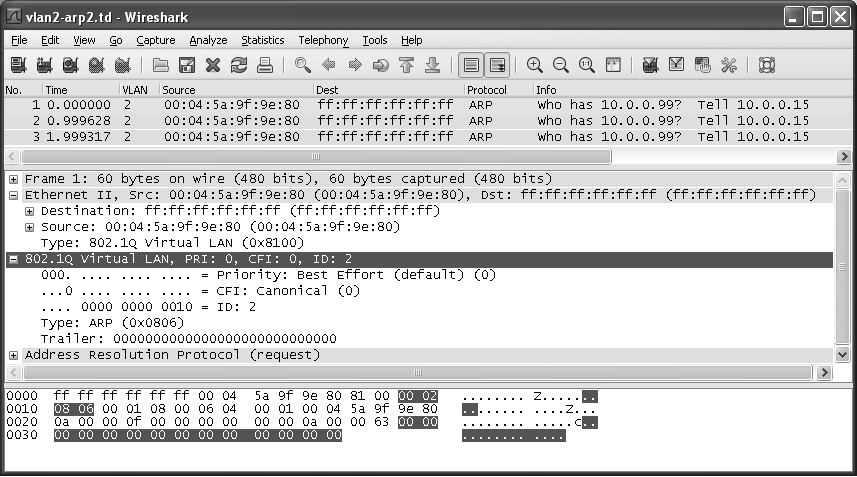
\includegraphics[scale=0.5]{imgs/3/3-5.png}
    \caption{VLAN ID 标记的帧显示在 Wireshark 中。默认的列和设置已被修改,以显示 VLAN ID 和原始以太网地址}
\end{figure}

本图显示了一个在 VLAN 2 中传输的ARP分组(见第4章)。我们可以看到,该帧大小
为60字节(不包括CRC)。该帧用 Ethernet II 封装(类型0x8100),表示一个 VLAN。另外
VLAN 头部表明该帧属于 VLAN2,优先级0,并且是普通帧。其他字段如我们预期的是
一个普通 ARP 分组。

\subsection{802.1AX:链路聚合(以前的802.3ad)}

有些系统配备多个网络接口,具有绑定(bonding)或链路聚合能力。通过链路聚合,
个或更多接口被视为一个,通过冗余或将数据分割(分拆)到多个接口,提高性能并获得更
好的可靠性。IEEE 修订的802.1AX[802.1AX-2008]定义了最常用的链路聚合方法,以及可
管理这些链路的链路聚合控制协议(LACP)。LACP 使用一种特定格式的IEEE 802帧(称为
LACPDU)。

以太网交换机支持的链路聚合是一个替代方案,它比支持更高速网络接口的性价比高。
如果多个端口聚合能提供足够的带宽,则可能并不需要高速接口。链路聚合不仅可被网络交
换机支持,而且可在一台主机上跨越多个网络接口卡(NIC)。在通常情况下,聚合的端口必
须是同一类型,并工作在同一模式(半双工或全双工)下。

Linux 可实现跨越不同类型设备的链路聚合(绑定),使用以下命令:
\begin{verbatim}
    Linux# modprobe bonding
    
    Linux# ifconfig bondo 10.0.0.111
    
    netmask 255.255.255.128
    
    Linux# ifenslave bondo ethO wlanO
\end{verbatim}

这组命令中的第一个用于加载绑定驱动,它是一个支持链路聚合的特设备驱动程序。

第二个命令使用IPv4地址来创建bondO接口。虽然IP 相关信息对创建聚合接口不是必需
的,但它是典型的。在ifenslave命令执行后,绑定设备bondO用MASTER 标志来标记,而
设备 ethO 和wlanO 用 SLAVE 标志来标记:
\begin{verbatim}
    bondo Link encap:Ethernet HWaddr 00:11:A3:00:2C:2A
    
    inet addr:10.0.0.111 Bcast:10.0.0.127 Mask:255.255.255.128
    
    inet6 addr: fe80::211:a3ff:fe00:2c2a/64 Scope:Link
    
    UP BROADCAST RUNNING MASTER MULTICAST MTU:1500 Metric:1
    
    RX packets:2146 errors:0 dropped:0 overruns:0 frame:0
    
    TX packets:985 errors:0 dropped:0 overruns:0 carrier:0
    
    col1isions:18 txgueuelen:0
    
    RX bytes:281939 (275.3 KiB)TX bytes:141391(138.0 KiB)
    
    ethO Link
    
    encap:Ethernet HWaddr 00:11:A3:00:2C:2A
    
    UP BROADCAST RUNNING SLAVE MULTICAST MTU: 1500 Metric:1
    
    RX packets:1882 errors:0 dropped:0 overruns:0 frame:0
    
    packets:961 errors:0 dropped:0 overruns:0 carrier:0
    
    collisions:18 txgueuelen:1000
    
    RX bytes: 244231 (238.5 KiB)TX bytes: 136561(133.3 KiB)
    
    Interrupt:20 Base address:0x6c00
    
    wlanO
    
    Link
    
    encap:Ethernet HWaddr 00:11:A3:00:2C:2A
    
    UP BROADCAST SLAVE MULTICAST MTU : 1500 Metric:1
    
    RX packets:269 errors:0 dropped:0 overruns:0 frame:0
    
    TX
    
    packets:24 errors:0 dropped: 0 overruns:0 carrier:0
    
    col1isions:0 txqueuelen: 1000
    
    RX bytes: 38579(37.6 KiB)™X bytes:4830 (4.7 KiB)
\end{verbatim}

在这个例子中,我们将一个有线以太网接口和一个Wi-Fi接口绑定在一起。为主设备
bondo 分配了 IPv4地址信息,通常分配给两个独立接口之一,它默认使用第一个从设备的
MAC地址。当IPv4流量通过bondO虚拟接日发送时,很可能使用不同的从设备来发送。在
Linux 中,当绑定的驱动程序被加载时,可使用系统提供的参数选择选项。例如,模式选
项决定了能否做以下工作:在接口之间使用循环交付,一个接口作为另一个接口的备份使
用,基于对MAC源地址和目的地址执行的异或操作选择接口,将帧复制到所有接口,执
行802.3ad标准的链路聚合,或采用更先进的负载平衡选项。第二种模式用于高可用性系
统,当一个链路停止运行时(由 MII 监控来检测;更多细节见[BOND]),这种系统将故障部
分转移到冗余的网络基础设施上。第三种模式是基于流量的流向选择从接口。如果目的地完
全不同,两个站之间的流量被固定到一个接口。在希望尽量少尝试重新排序,并保证多个接
口负载平衡的情况下,这种模式可能是有效的。第四种模式针对容错。第五种模式用于支持
802.3ad 的交换机,在同类链路上实现动态聚合能力。

LACP 协议旨在通过避免手工配置,以简化链路聚合的建立工作。在LACP “主角”(客
户端)和“参与者”(服务器)启用后,它们通常每秒都会发送LACPDU。LACP 自动确定哪
些成员链路可被聚合成一个链路聚合组(LAG),并将它们聚合起来。这个过程的实现需要通
过链路发送一系列信息(MAC地址、端口优先级、端口号和密钥)。一个接收站可比较来自
其他端口的值,如果匹配就执行聚合。LACP 协议的细节见[802.1AX-2008]。

\section{全双工、省电、自动协商和 802.1X流量控制}

当以太网最初被开发出来时,它仅工作在半双工模式,并使用一条共享的电缆。也就是
说,同一时间内只能在一个方向发送数据,因此在任何时间点只有一个站可发送一个帧。随着
交换式以太网的发展,网络不再是单一的共享线路,而代之以很多链路的组合。因此,多个站
之间可以同时进行数据交换。另外,以太网被修改为全双工操作,这样可以有效禁用冲突检测
电路。这样也可以增加以太网的物理长度,因为半双工操作和冲突检测的相关时间约束被取消。
在 Linux 中,ethtool 程序可用于查询是否支持全双工,以及是否正在执行全双工操作。

这个工具也可显示和设置以太网接口的很多属性:

\begin{verbatim}
    Linux# ethtool ethO
    
    Settings for ethO:
    
    Supported ports: [ TP MII ]
    
    Supported link modes: 10baseT/Half 10baseT/Fu11
    
    100baseT/Half 100baseT/Fu11
    
    Supports
    
    auto-negotiation: Yes
    
    Advertised link modes: 10baser/Half 10baser/Fu11
    
    100baseT/Half 100baser/Fu11
    
    Advertised auto-negotiation: Yes
    
    Speed: 10Mb/s
    
    Duplex:Half
    
    Port: MII
    
    PHYAD: 24
    
    Transceiver: internal
    
    Auto-negotiation: on
    
    Current message level: 0x00000001 (1)
    
    Link detected: yes
    
    Linux# ethtool eth1
    
    Settings for ethl:
    
    Supported ports:[ TP]
    
    Supported 1ink modes: 10baser/Half 10baser/Fu11
    
    100baser/Half 100baseT/Fu11
    
    1000baser/Fu11
    
    Supports auto-negotiation: Yes
    
    Advertised link modes: 10baseT/Half 10baser/Fu11
    
    100baser/Half 100baser/Fu11
    
    1000baseT/Fu11
    
    Advertised auto-negotiation: Yes
    
    Speed: 100Mb/s
    
    Duplex: Fu11
    
    Port: Twisted Pair
    
    PHYAD:0
    
    Transceiver: internal
    
    Auto-negotiation: on
    
    Supports Wake-on: umba
    
    Current message level:0x00000007 (7)
    
    Link
    
    detected: yes
\end{verbatim}

在这个例子中,第一个以太网接口(ethO)连接到一个半双工的10Mb/s网络。我们看到
它能够自动协商,这是一种来源于802.3u的机制,使接口能交换信息(例如速度)和功能
(例如半双工或全双工运行)。自动协商信息在物理层通过信号交换,它可在不发送或接收数
据时发送。我们可以看到,第二个以太网接口

Intel(R) 82577LN Gigabit Network Connection Properties

(ethl)也支持自动协商,它的速率100Mb/

S,工作模式为全双工。其他值(Port、

PHYAD、Transceiver) 指出物理端口类型、地

址,以及物理层电路在NIC内部还是外部。

当前消息级别用于配置与接口操作模式相关的

日志消息,它的行为由使用的驱动程序指定。

我们在下面的例子讨论如何设置这些值。

在Windows 中,我们可以看到以下细节,

首先进入“控制面板”中的“网络连接”,然

Adaptive Irter-Frame Spacing

Enable PME

Flow Control

Gigabi Master Slave Mode

Intemupt Moderation

hntemupt Moderation Rate

IPy4 Checksum Ofload

Jumbo Packet

Large Send Oiioad (IPv4)

Lare Send OHiload(Py5)

Link Speed Battery Saver

Locakly Administered Address

LLog Link State Evert

Autto Negotiation

1.0Gops Fu Duple

10 Mbps Ful Duplex

10 Mbps Half Duplex

100 Mbps Fuil Duplex

100 Mos Half Dupdex

后在感兴趣的接口上单击鼠标右键并选择“属性”,然后单击“配置”框并选择“高级”选
项卡。这时,将打开一个类似图3-6(这个例子来自 Windows 7机器上的以太网接口)所示
的对话框。

在图3-6中,我们可看到通过适配器的设备驱动程序来配置的特殊功能。对于这个特殊
的适配器和驱动程序,802.1p/q 标签可启用或禁用,也可提供流量控制和唤醒功能
(见3.3.2节)。我们可以手工设置速率和双工模式,或使用更典型的自动协商选项。

驱动程序的运行参数

\begin{figure}
    \centering
    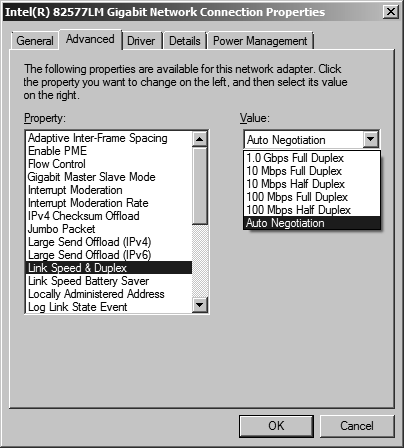
\includegraphics[scale=0.5]{imgs/3/3-6.png}
    \caption{Windows (7)的网络接口属性的“高级”选项卡。该控件允许用户提供网络设备}
\end{figure}

\subsection{双工不匹配}

自动协商曾经有一些互操作性问题,特别是一台计算机及其相关的交换机端口使用不同
的双工配置时,或者当自动协商只在链路的一端被禁用时。在这些情况下,可能会发生双工
不匹配。令人惊讶的是,当这种状况发生时,连接不会完全失败,但可能带来显著的性能下
降。当网络中出现中等程度的双向流量繁忙时(例如,在大数据传输期间),一个半双工接口
会将输入的流量检测为冲突,从而触发以太网MAC的CSMA/CD 的指数退避功能。同时,
导致这个冲突的数据被丢弃,这可能需要更高层协议(例如 TCP)重传。因此,性能下降可
能只在半双工接口发送数据,同时又有大量流量需要接收时才是明显的,站处于轻负载时通
常不会发生这种情况。一些研究者已试图开发分析工具来检测这种问题[SCO5]。

\subsection{局域网唤醒(WoL)、省电和魔术分组}

在 Linux 和 Windows 的例子中,我们看到一些电源管理方面的功能。Windows 唤醒功能
和Linux 唤醒选项用于使网络接口或主机脱离低功耗(睡眠)状态,这是基于某类分组的传输
来实现的。这种分组用来触发可配置的功率状态改变。在Linux 中,用于唤醒的值可以是零
或者是多个用于低功耗状态唤醒的位,它们可以被以下几种帧所触发:任何物理层(PHY)活
动(p)、发往站的单播帧(u)、组播帧(m)、广播帧(b)、ARP帧(a)、魔术分组帧(g),以及
包括密码的魔术分组帧。这些都可以使用 ethtool 的选项来配置。例如,可以使用以下命令:

\begin{verbatim}
    Linux# ethtool -s etho wol umgb
\end{verbatim}

当接收到任何u、m、g或b类型的帧时,这个命令将 etho设备配置为发送一个唤醒信
号。Windows 提供了类似的功能,但标准的用户接口只支持魔术分组帧,以及一个预定义的
u、m、b 和a类型帧的子集。魔术分组包含一个字节值 OxFF 的特定重复模式。在通常情况下,
这种帧采用 UDP 分组(见第10章)形式封装在以太网广播帧中发送。有几个工具可以生成
它们,包括 wol[WOL]:

\begin{verbatim}
    Linux# wol 00:08:74:93:C8:3C
    Waking up 00:08:74:93:C8:3C.
\end{verbatim}

这个命令的结果是构造一个魔术分组,我们可以使用 Wireshark 查看(见图3-7)。

\begin{figure}
    \centering
    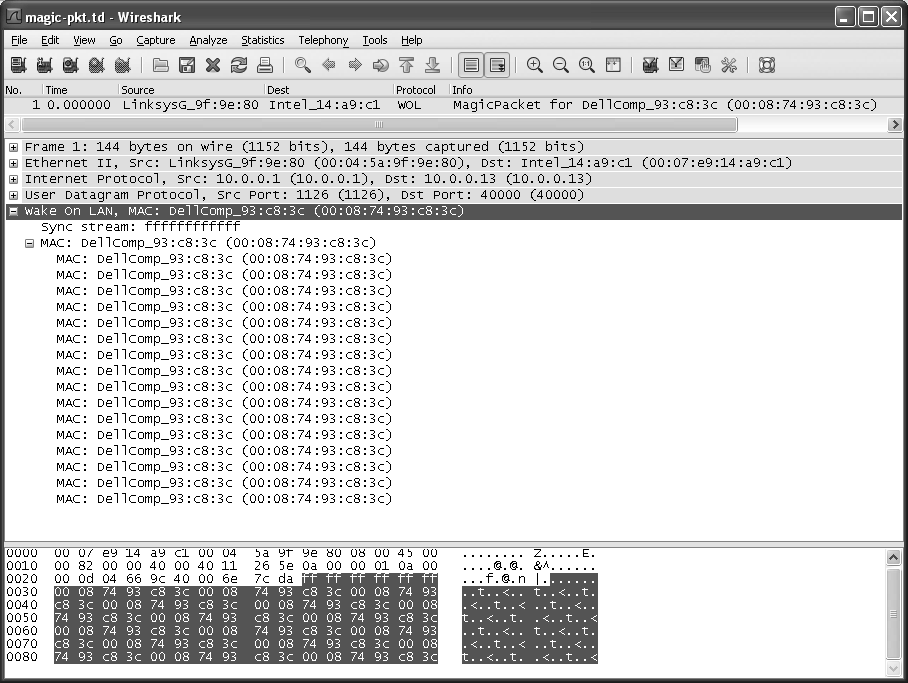
\includegraphics[scale=0.5]{imgs/3/3-7.png}
    \caption{Wireshark 中的一个魔术分组帧,开始是6字节的 OxFF,然后重复 MAC地址16次}
\end{figure}

图3-7中显示的分组多数是传统的UDP 分组,但端口号(1126和40000)是任意的。
分组中最特别的是数据区域。它以一个6字节的值OxFF 开始,其余部分包含重复16次的目
的MAC地址 00:08:74:93:C8:3C。该数据的有效载荷模式定义了魔术分组。

\subsection{链路层流量控制}

以全双工模式运行扩展的以太网和跨越不同速率的网段时,可能需要由交换机将帧缓
存(保存)一段时间。例如,当多个站发送到同一目的地(称为输出端口争用),这种情况可
能发生。如果一个站聚合的流量速率超过该站的链路速率,那么帧就开始存储在中间交换机
中。如果这种情况持续一段时间,这些帧可能被丢弃。

缓解这种情况的一种方法是在发送方采取流量控制(使它慢下来)。一些以太网交换机
(和接口)通过在交换机和网卡之间发送特信号帧来实现流量控制。流量控制信号被发送
到发送方,通知它必须放慢传输速率,但规范将这些细节留给具体实现来完成。以太网使用
PAUSE 消息(也称为 PAUSE 帧)实现流量控制,它由802.3x[802.3-2008]来定义。

PAUSE 消息包含在MAC控制帧中,通过将以太网长度/类型字段值设为0x8808,以及
使用MAC控制操作码0x0001来标识。如果一个站接收到这种帧,表示建议它减缓发送速
度。PAUSE 帧总是被发送到 MAC地址 01:80:C2:00:00:01,并且只能在全双工链路上使用。
它包含一个保持关闭(hold-off)时间值(指定量为512比特的时间),表明发送方在继续发送
之前需要暂停多长时间。

MAC控制帧采用如图3-3所示的常规封装的帧格式,但紧跟在长度/ 类型字段后的是一
个2字节的操作码。PAUSE 帧实际上是唯一一种使用MAC控制帧的帧类型。它包括一个2
字节的保持关闭时间。“整个”MAC控制层(基本只是802.3x 流量控制)的实现是可选的。

以太网层次的流量控制可能有重大负面影响,因此通常并不使用它。当多个站通过一台
过载的交换机发送时(见下一节),该交换机通常向所有主机发送 PAUSE 帧。不幸的是,交
换机的内存使用可能对发送主机不均衡,因此有些主机可能被惩罚(流量控制),即使它们对
交换机流量过载没有多少责任。

\section{网桥和交换机}

IEEE 802.1d 标准规定了网桥的操作,交换机本质上是高性能的网桥。网桥或交换机用
于连接多个物理的链路层网络(例如一对物理的以太网段)或成组的站。最基本的设置涉及
连接两个交换机来形成一个扩展的局域网,如图3-8所示。

图3-8 一个包括两台交换机的扩展以太网。每个交换机端口有一个编号,
每个站(包括每个交换机)有自己的MAC地址

图中的交换机 A 和B互连形成一个扩展的局域网。在这个特定例子中,客户端系统都
连接到A,服务器都连接到B,端口编号供参考。注意,每个网络单元(包括每个交换机)
有自己的MAC地址。每个网桥经过一段时间对域外 MAC地址的“学习”后,最终每个交
换机会知道每个站可由哪个端口到达。每个交换机基于每个端口(也可能是每个 VLAN)的
列表被存储在一张表(称过滤数据库)中。图3-9显示每个交换机了解每个站的位置后,
形成的包含这些信息的数据库例子。

当第一次打开一个交换机(网桥)时,它的数据库是空的,因此它不知道除自己之外的
任何站的位置。当它每次接收到一个目的地不是自己的帧时,它为除该帧到达的端口之外的
所有端口做一个备份,并向所有端口发送这个帧的备份。如果交换机(网桥)未学习到站的
位置,每个帧将会被交付到每个网段,这样会导致不必要的开销。学习能力可以显著降低开
销,它是交换机和网桥的一个基本功能。

图 3-9

站

00:17:f2:a2:10:3d

00:c0:19:33:0a:2e

端口

2

1

站

00:17:f2:a2:10:3d

00:c0:19:33:0a:2e

00:0d:66:4f:02:03

00:0d:66:4f:02:03

端口

9

9

9

00:0d:66:4f:02:04

00:30:48:2b:19:82

00:30:48:2b:19:86

3

3

3

00:0d:66:4f:02:04

00:30:48:2b:19:82

00:30:48:2b:19:86

0I

11

交换机A的数据库

交换机B的数据库

交换机 A和B 中的过滤数据库是从图3-8经过一段时间“学习”,

通过查看交换机端口上的帧的源地址来创建

目前,多数操作系统支持网络接口之间的网桥功能,这意味着具有多个接口的计算机
可用作网桥。例如,在Windows 中,多个接口可被桥接,进人“控制面板”的“网络连接”
菜单,选中(突出显示)需要桥接的接口,点击鼠标右键,并选择“网桥连接”。这时,出
现一个表示网桥功能的新图标。许多接口相关的正常网络属性消失,取而代之的是网桥设备
(见图3-10)。

\begin{figure}
    \centering
    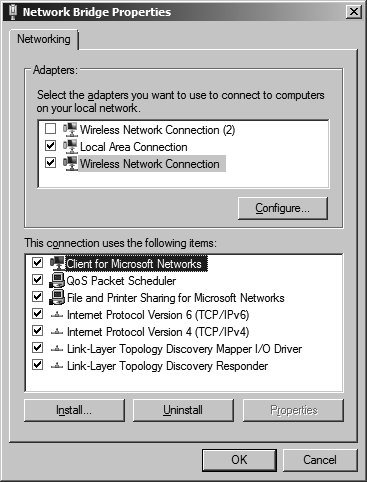
\includegraphics[scale=0.5]{imgs/3/3-10.png}
    \caption{在 Windows 中,通过选中需要桥接的网络接口,鼠标右击并选择桥接网络接口,可创建网桥设备。在网桥建立之后,可进一步修改网桥设备}
\end{figure}

图3-10显示 Windows 7 中的虚拟网桥设备的属性面板。网桥设备的属性包括一个被桥
接的相关设备列表,以及在网桥上运行的一组服务(例如,Microsoft 网络客户端、文件和打
印机共享等)。Linux 以类似方式工作,它使用命令行参数。在这个例子中,我们使用图3-11
所示的拓扑结构

图 3-11
在这个简单的拓扑中,一台基于Linux 的PC被配置网桥,它在两个以太网之间实现互联。
作为一个处于学习中的网桥,它不断积累并建立一些表,其中包含有关哪个端口可到达扩展
局域网中的其他系统的信息

在图3-11中,这个简单的网络使用一台基于Linux、带两个端口的PC作为网桥。只有
一个站连接到端口2,网络其他部分都连接到端口1。以下命令可启用网桥:
\begin{verbatim}
    Linux# brctl addbr bro
    Linux# brctl addif bro eth0
    Linux# brctl addif bro eth1
    Linux# ifconfig eth0 up
    Linux# ifconfig eth1 up
    Linux# ifconfig bro up
\end{verbatim}

以下几个命令可创建一个网桥设备brO,并网桥增加接口 ethO 和 ethl。brctl delif 命令
可用于删除接口。在建立接口之后,brctl showmacs 命令可用于检查过滤数据库(称转发
数据库,用Linux 的术语称为 fdbs):

\begin{verbatim}
    Linux# brctl show
    bridge name bridge id         STP enabled interfaces
    brO         8000.0007e914a9cl no          etho ethl
    
    Linux# brctl showmacs br0
    port no mac addr is local? ageing timer
        1 00:04:5a:9f:9e:80 no 0.79
        2 00:07:e9:14:a9:cl yes 0.00
        1 00:08:74:93:c8:3c yes 0.00
        2 00:14:22:f4:19:5f no 0.81
        1 00:17:f2:e7:6d:91 no 2.53
        1 00:90:£8:00:90:b7 no 17.13
\end{verbatim}

这个命令的输出显示关于网桥的其他细节。由于站可能出现移动、网卡更换、MAC地
址改变或其他情况,所以就算网桥曾发现一个 MAC地址可通过某个端口访问,这个信息也
不能假设永远是正确的。为了解决这个问题,在每次学习一个地址后,网桥启动一个计时器
(通常默认5分钟)。在Linux 中,每个学习条目使用一个与网桥相关的固定时间。如果在
指定的“有效期”内,没有再次看到该条目中的地址,则将这个条目删除,如下所示:

\begin{verbatim}
    Linux# brctl setageing bro 1
    Linux# brctl showmacs br0 port no
    
    mac addr is local? ageing
    
    timer
    
    1 00:04:5a:9f:9e:80 no 0.76
    2 00:07:€9:14:a9:c1 yes 0.00
    1 00:08:74:93:c8:3c yes 0.00
    2 00:14:22:f4:19:5f no 0.78
    1 00:17:f2:e7:6d:91 no 0.00
\end{verbatim}

为了方便演示,我们选择了一个比平时数值低的值作为有效期。当一个条目因有效期满
而被删除时,后续的帧将被发送到接收端口之外的所有端口(称为洪泛),并更新过滤数据库
中的这个条目。实际上,过滤数据库的使用和学习有利于优化性能,如果表是空的,网络将
花费更多开销,但仍能履行职责。下一步,我们将注意力转移到两个以上的网桥通过冗余链
路互联的情况。在这种情况下,帧的洪泛可能导致帧永远循环的洪泛灾难。显然,我们需要
一种方法来解决这个问题。

\subsection{生成树协议}

网桥可能单独或与其他网桥共同运行。当两个以上的网桥使用(或交换机端口交叉连接)
时,由于存在级联的可能性,因此可能形成很多组的循环帧。我们看如图3-12所示的网络。

假设图3-12中的多个交换机刚被打开,并且它们的过滤数据库为空。当站S发送一个
帧时,交换机B在端口7、8和9复制该帧。这时,最初的帧已被“放大”3倍。这些帧被
交换机 A、D和C接收。交换机 A在端口2和3生成该帧的副本。交换机 D和C分别在端
口 20、22和13、14生成更多副本。当这些

交换机A

副本在交换机 A、C和D之间双向传输,这

时放大倍数已增大为6。当这些帧到达时,

转发数据库开始出现震荡,这是由于网桥反

复尝试查找通过哪些端口可到达站S。显然,

21

这种情况是不能容忍的。如果允许这种情况

交换机B

站S

20

交换机D

发生,采用这种配置的网桥将无法使用。幸

12

运的是,有一种协议可避免这种情况,这种

协议称生成树协议(STP)。我们将介绍

图3-12

STP的一些细节,解释网桥和交换机采用哪

些方法抑制放大。在当前的标准[802.1D-

2004]中,传统的STP被快速生成树协议

(RSTP)代替,我们将在了解传统STP的基

14

交换机C

一个扩展的以太网包括4台交换机和多

条冗余链路。如果在这个网络中采用简单

的洪泛转发帧,由于多余的倍增流量(所

谓的广播风暴),将会导致一场大的灾难。

这种情况需要使用 STP

础上再介绍它。

STP通过在每个网桥禁用某些端口来工

交换机A

1

作,这样可避免拓扑环路(即两个网桥之间

不允许出现重复路径),但如果拓扑结构未分

区,则仍可到达所有站。在数学上,一个生

6

21

成树是一张图中所有节点和一些线的集合,

交换机B

13

从任何节点到其他节点(跨越图)有一条路径

站S

交换机D

12

或路由,但是没有环路(这些线的集合构成
一棵树)。一张图可能存在多个生成树。STP
用于找出这张图的其中一个生成树,该图将
网桥作为节点并将链路作为线(或称“边”)。

图3-13说明了这个想法。

在本图中,粗线表示网络中被STP选择

用于转发帧的链路。其他链路没有被使用,

端口8、9、12、21、22和3被阻塞。通过

14

交换机C

图3-13

通过STP,链路B-A、A-C和C-D在生

成树中是活跃的。端口6、7、1、2、13、

14和20处于转发状态;所有其他端口被

阻塞(即不转发)。这样可以防止帧循环,

避免广播风暴。如果配置发生变化或某台

交换机故障,则将阻塞端口改变为转发状

态,并由网桥计算一个新生成树

使用STP,早期的各种问题并没有出现,这些帧只是作为另一个抵达帧的副本而被创建。这
里没有出现放大的问题。由于任意两个站之间只有一条路径,因此可以避免循环。生成树的
形成和维护由多个网桥完成,在每个网桥上运行一个分布式算法。

用于转发数据库时,STP必须处理以下情况,例如网桥启用和关闭、接口卡更换或
MAC地址改变。显然,这种变化可能影响生成树运行,因此STP 必须适应这些变化。这种
适应通过交换一种称为网桥协议数据单元(BPDU)的帧来实现。这些帧用来形成和维护生
成树。这棵树“生长”自一个网桥——该网桥由其他网桥选举为“根网桥”。

如前所述,一个网络可能存在多个生成树。如何确定哪棵生成树最适于转发帧,这基于
每条链路和根网桥位置的相关成本。这个成本是一个与链路速度成反比的整数(建议)。例
如,一条10Mb/s链路的成本为100,100Mb/s 和 1000Mb/s链路的成本分别为19和4。STP
计算到根网桥的成本最小的路径。如果必须遍历多条链路,相关成本是这些链路成本之和。

\subsubsection{端口状态和角色}

为了理解STP的基本操作,我们需要了解网桥端口的状态机,以及BPDU 内容。网桥
端口可能有5个状态:阻塞、侦听、学习、转发和禁用。在图3-14所示的状态转换图中,我
们可以看出它们之间的关系。

拓扑改变

初始化

阻塞

(丟弃)

最大

一时间

(20s)

侦听

(丟弃)

转发

一延迟一

(15s)

学习

转发

转发延迟

(15s)

拓扑改变

禁用

(丢弃)

拓扑改变

图3-14
在正常的STP操作中,端口在4个主要状态之间转换。在阻塞状态下,帧不被转发,但一次
拓扑变化或超时可能导致向侦听状态转换。转发状态是活跃的交换机端口承载数据流量的正
常状态。括号中的状态名用于表示 RSTP 相关的端口状态

在图3-14显示的生成树中,实线箭头表示端口的正常转换,小的虚线箭头表示由管理
配置引起的改变。在初始化后,一个端口进人阻塞状态。在这种状态下,它不进行地址学
习、数据转发或 BPDU 发送,但它会监控接收的BPDU,并在它需要被包含在将到达的根
网桥的路径中的情况下,使端口转换到侦听状态。在侦听状态下,该端口允许发送和接收
BPDU,但不进行地址学习或数据转发。经过一个典型的15秒的转发延迟,端口进入学习状
态。这时,它被允许执行数据转发之外的所有操作。在进入转发状态并开始转发数据之前,
需要等待另一个转发延迟。

相对于端口状态机,每个端口都扮演一定的角色。由于RSTP(见3.4.1.6节)的出现,
这个术语变得越来越重要。端口可能扮演根端口、指定端口、备用端口或备份端口等角色。
根端口是生成树中位于指向根的线段终点的那些端口。指定端口是指处于转发状态,并与根
相连线段中路径成本最小的端口。备用端口是与根相连线段中成本更高的端口。它们不处于
转发状态。备份端口是指连接到同一线段中作为同一网桥指定端口使用的端口。因此,备份
端口可轻易接管一个失效的指定端口,而不影响生成树拓扑的其余部分,但是它不能在全部
网桥失效的情况下提供一条到根的备用路径。

\subsubsection{ BPDU 结构}

为了确定生成树中的链路,STP 使用图3-15所示的BPDU。

帧

前导

SFD

(7字节)(1)

DST

(6)

SRC

(6

LLC/

L/T

Prot Vers Type Flags

SNAP

(2

(3

2)

(1)

(1

(1)

根1

(⑧

BPDU

根路径

网桥1D

成本

(4)

(8

(2)

2

Hello 转发

Mah

Time延迟

(2)

FCS

(4)

(1 (1(2位)(1)(1)(1)

由802.1w

定义

图3-15
BPDU 被放置在802帧的有效载荷区,并在网桥之间交换以建立生成树。重要的字段包括
源、根节点、到根的成本和拓扑变化提示。在802.1w 和[802.1D-2004]中(包括快速 STP或
RSTP),附加学段显示端口状态

图3-15所示的格式适用于最初的STP,以及新的RSTP(见3.4.1.6节)。BPDU 总被发送
到组地址 01:80:C2:00:00:00(链路层组和因特网组播寻址的详细信息见第9章),并且不会通过
一个未修改的网桥转发。在该图中,DST、SRC 和L/T(长度/类型)字段是携带 BPDU 的传
统以太网(802.3)帧头部的一部分。3字节的LLC/SNAP头部由802.1定义,并针对BPDU 被
设置为常数Ox424203。并非所有BPDU 都使用 LLC/SNAP 封装,但这是一个常见的选项。

协议(Prot)字段给出协议ID 号,它被设置次0。版本(Vers)字段被设置为0或2,取
决于使用STP还是RSTP。类型(Type)字段的分配与版本类似。标志(Flags)字段包含拓
扑变化(TC)和拓扑变化确认(TCA)位,它们由最初的802.1d 标准定义。附加位被定义为
建议(P)、端口角色(00为未知,01备用,10为根,11为指定)、学习(L)、转发(F)和
协议(A)。这些都作为 RSTP 内容在3.4.1.6节中讨论。根 ID 字段给出发送方使用的根网桥
标识符,即从网桥ID 字段中获得的MAC地址。这些ID 字段都用一种特方式编码,包
括MAC地址之前的一个2字节的优先级字段。优先级的值可通过管理软件来设置,以强制
要求生成树采用某个特定网桥作为根(例如,Cisco 在自己的Catalyst 交换机中使用默认值
0x8000)。

根路径成本是在根ID字段中指定的计算出的到达某个网桥的成本。PID 字段是端口
标识符和由发送帧给出的端口号,它被附加在一个可配置的1字节的优先级字段(默认力
0x80)之后。消息有效期(MsgA)字段指出消息有效期。最大有效期(MaxA)字段指出超
时(默认为20秒)的最大期限。欢迎时间(Hello Time)字段指出配置帧的传输周期。转发
延迟字段指出处于学习和侦听状态的时间。所有的有效期和时间字段可在1/256秒内获得。

消息有效期字段不像其他的时间字段那样是固定值。当根网桥发送一个 BPDU时,它将
该字段设置为0。网桥转发接收到的不是根端口的帧,并将消息有效期字段加1。从本质上
来说,该字段是一个跳步计数器,用于记录BPDU 经过的网桥数量。当一个 BPDU 被一个
端口接收时,其包含的信息在内存和STP算法参与者中被保存至超时(超时发生在(MaxA-
MsgA)时刻)。如果超过这个时间,根端口没有接收到另一个 BPDU,根网桥被宣布“死亡”,
并重新开始根网桥选举过程。

\subsubsection{建立生成树}

STP 的第一个工作是选举根网桥。根网桥是在网络(或VLAN)中标识符最小(优先级与
MAC地址结合)的网桥。当一个网桥初始化时,它假设自己是根网桥,并用自己的网桥ID 作
为根ID 字段的值发送配置BPDU消息,如果它检测到一个ID 更小的网桥,则停止发送自己
的帧,并基于接收到的ID 更小的帧构造下一步发送的BPDU。发出根ID 更小的BPDU 的端
口被标记为根端口(即端口在到根网桥的路径上)。剩余端口被设置为阻塞或转发状态。

\subsubsection{拓扑变化}

STP 的另一个重要工作是处理拓扑变化。虽然可用前面所述的数据库有效期机制适应拓扑
变化,但这是一个比较差的方法,因为有效期计时器需要花费很长时间(5分钟)删除错误条
目。相反,STP 采用一种方法检测拓扑变化,并快速通知它们所在的网络。在STP中,当一
个端口进入阻塞或转发状态时,意味着发生拓扑变化。当网桥检测到一个连接变化(例如一条
链路故障),它向根端口之外的端口发送拓扑变化通知(TCN)BPDU,通知自己在树中的父网
桥,直到根止。树中通向根的下一个网桥向发送通知的网桥确认 TCNBPDU,并将它们转
发到根。当接收到拓扑变化通知时,根网桥在后续的周期性配置消息中设置TC位。这种消息
被网络中的每个网桥所转发,并被处于阻塞或转发状态的端口接收。设置这个位允许网桥减小
转发延时计时器的有效期,将有效期以秒代替推荐的5分钟。这样,数据库中已有的错误条目
可被快速清除和重新学习,同时允许访问那些被误删除的条目。

\subsubsection{例子}

在 Linux 中,网桥功能默认禁用STP。假设在多数情况下拓扑相对简单,一台普通计算
机可被用作网桥。可执行以下命令为当前使用的网桥启用 STP:

\begin{verbatim}
    Linux# brctl str bro on
\end{verbatim}

执行该命令的结果如下:

\begin{verbatim}
    Linux# brctl showstr bro
    
    bro
    
    bridge id
    
    designated root
    
    root port
    
    max age
    
    hello time
    
    forward delay
    
    ageing time
    
    hel10 timer
    
    topology change timer
    
    8000.0007e914a9c1
    
    8000.0007e914a9c1
    
    0
    
    19.99
    
    1.99
    
    14.99
    
    0.99
    
    1.26
    
    3.37
    
    path cost
    
    bridge max age
    
    bridge hello time
    
    bridge forward delay
    
    tcn timer
    
    gc timer
    
    0
    
    19.99
    
    1.99
    
    14.99
    
    0.00
    
    3.26
    
    flaas
    
    TOPOLOGY CHANGE TOPOLOGY CHANGE DETECTED
    
    etho (0)
    
    port id
    
    designated root
    
    designated bridge
    
    designated port
    
    designated cost
    
    0000
    
    8000.0007e914a9c1
    
    8000.0007e914a9c1
    
    8001
    
    o
    
    state
    
    forwarding
    
    path cost
    
    100
    
    message age timer
    
    0.00
    
    forward delay timer 0.00
    
    hold timer
    
    0.26
    
    flags
    
    ethi (0)
    
    port id
    
    designated root
    
    designated bridge
    
    designated port
    
    designated cost
    
    0000
    
    8000.0007e914a9c1
    
    8000.0007e914a9c1
    
    8002
    
    0
    
    state
    
    Eorwarding
    
    path cost
    
    19
    
    message age timer
    
    0.00
    
    forward delay timer 0.00
    
    hold timer
    
    0.26
    
    flags
\end{verbatim}

我们看到一个简单的桥接网络的STP设置。网桥设备br0保存网桥的整体信息。这些信
息包括网桥ID(8000.0007e914a9c1),它由图3-11 中基于PC的网桥(端口 1)的最小MAC
地址生成。可在几秒钟内获得主要的配置参数(例如欢迎时间、拓扑变化计时器等)。标志
值表示最近的拓扑变化,用于获得最近的网络连接变化的实际情况。输出的其余部分描述每
个端口的信息,即ethO(网桥端口 1)和 ethl(网桥端口2)。注意,ethO的路径成本大约是
ethl成本的10倍。这个结果与 etho 是一个 10Mb/s 以太网而 ethl是一个100Mb/s 全双工网
络是一致的。

我们可使用 Wireshark查看一个BPDU。在图3-16中,我们看到一个52字节的消息内
容。消息长度52字节(由于Linux捕获功能会拆除填充,因此它小于以太网的64字节
的最小限制),这个长度是由以太网头部中的长度/类型字段加14得到的。目的地址是预期
的组地址01:80:C2:00:00:00。有效载荷长度是38字节,这个值包含在长度字段中。SNAP/
LLC字段包含常数0x424243,并且封装帧是一个生成树(版本0)帧。其余协议字段表明
站 00:07:e9:14:a9:c1 认为自己是生成树的根,优先级为32768(低优先级),并且 BPDU从
端口2以优先级 0x80发送。另外,最大有效期是20秒,欢迎时间是2秒,转发延迟是
15秒。

\subsubsection{快速生成树协议(以前的 802.1w)}

传统STP 的问题之一是在拓扑变化之后,只能通过一定时间内未接收到 BPDU 来检测。
如果这个超时很大,收敛时间(沿着生成树重新建立数据流的时间)可能比预期大。IEEE
802.1w 标准([802.1D-2004] 的一部分)改进了传统STP,它定义了采用新名称的快速生成树
协议(Rapid Spanning Tree Protocol,RSTP)。在RSTP 中,对STP的主要改进是监视每个端
口的状态,并在故障时立即发送一个拓扑变化通知。另外,RSTP使用BPDU 的标志字段中
的全部6位来支持网桥之间的协议,以避免由计时器来启动协议操作。它将正常的STP端口
状态由5个减少到3个(丢弃、学习和转发,由图3-14的括号中的状态名表示)。RSTP的
丢弃状态代替了传统STP 的禁止、阻塞和侦听状态。RSTP 创建了一个称为备用端口的新角
色,作用是在根端口停止运行时立即代替它。

由于RSTP 只使用一种类型的BPDU,因此这里没有专门的拓扑变化BPDU。正如所说
的那样,RSTP 的BPDU 使用版本和类型号2而不是0。在RSTP 中,检测到一次拓扑变化
的交换机会发送一个表示拓扑变化的BPDU,任何接收到它的交换机立即清除自己的过滤数
据库。这个改变可显著影响协议的收敛时间。这时,无须等待拓扑变化传递到根网桥再经过
转发延迟后返回,而是立即清除相关条目。总之,在大多数情况下,收敛时间可从几十秒减
少到几分之一秒。

\begin{figure}
    \centering
    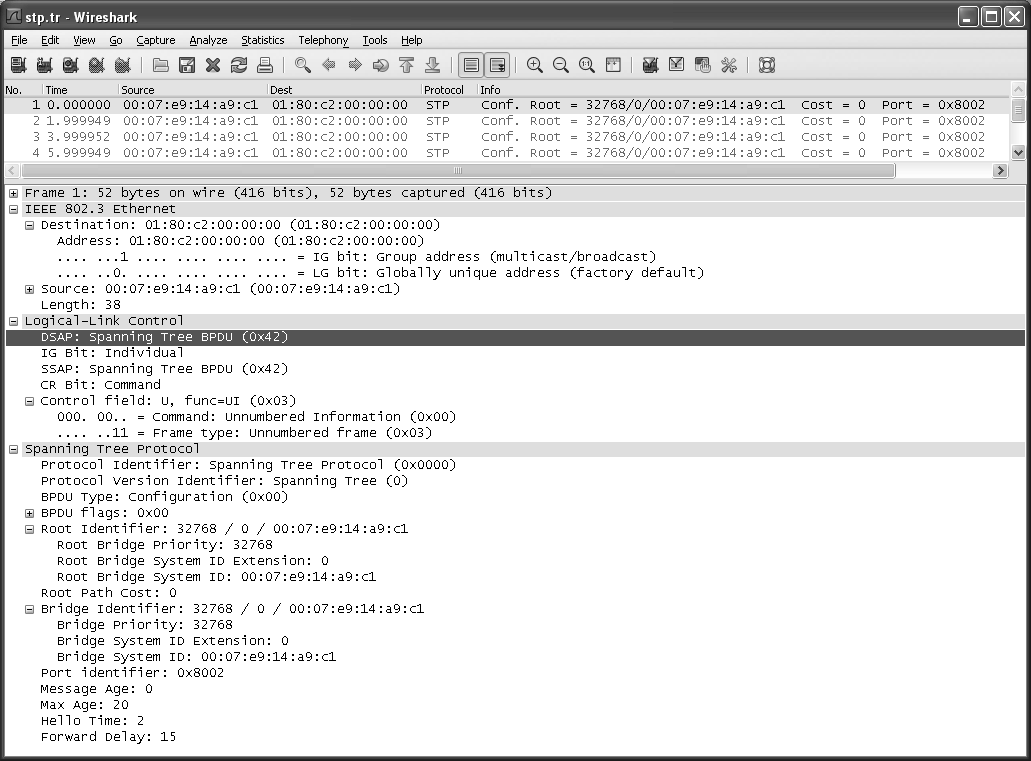
\includegraphics[scale=0.5]{imgs/3/3-16.png}
    \caption{Wireshark 显示一个 BPDU。以太网帧的目的地址是一个通过网桥(01:80:c2:00:00:00)的组地址}
\end{figure}

RSTP 使边缘端口(只连接到端站的端口)和正常的生成树端口之间,以及点到点链路
和共享链路之间都有区别。边缘端口和点到点链路上的端口通常不会形成循环,因此允许它
们跳过侦听和学习状态,直接进入转发状态。当然,如果假设一个边缘端口可能被入侵,例
如两个端口交叉连接,它们可携带任何形式的BPDU(简单的端站通常不处理 BPDU),这时
它们将被重新分类为生成树端口。点到点链路可根据接口操作模式来识别。如果这个接口运
行在全双工模式下,则这条链路是点到点链路。

在普通的STP 中,BPDU通常由一个通知网桥或根网桥来转发。在 RSTP 中,BPDU *
了“保持活跃”而由所有网桥来定期发送,以便确定相连的邻居是否正常运行。大多数高层
路由协议也会这样做。注意,在RSTP 中,拓扑变化没有像普通STP那样包括边缘端口连接
或断开。当检测到一次拓扑变化时,通知网桥发送TC位被设置的BPDU,不仅到根网桥而
且到所有网桥。这样做允许将拓扑变化通知整个网络,并且比传统STP 更快速。当一个网桥
接收到这些消息时,它会更新除边缘端口之外的所有相关条目。

RSTP 的很多功能由 Cisco和其他公司开发,他们有时需要在自己的产品中为普通STP
做专门的扩展。IEEE 委员会将这些扩展纳人802.1d标准的更新中,该标准涵盖所有类型的
STP,因此扩展局域网可在某些网段中运行传统STP,同时在其他部分中运行 RSTP(虽然
RSTP 的优势将丧失)。RSTP已被扩展到 VLAN[802.1Q-2005]中,它采用一种称多生成
树协议(MSTP)的协议。这个协议保留了 RSTP(和STP)报文格式,因此它有可能做到向
后兼容,也支持形成多个生成树(每个 VLAN一个生成树)。

\subsection{802.1ak:多注册协议}

多注册协议(Multiple Registration Protocol, MRP) 提供了在桥接局域网环境中的站之
间注册属性的通用方法。[802.1ak-2007]定义了两个特殊的MRP“应用程序”,称次MVRP
(用于注册 VLAN)和 MMRP(用于注册组 MAC地址)。MRP 代替了早期的GARP框架;
MVRP 和 MMRP 分别代替了旧的GVRP 和GMRP协议。这些协议最初都由 802.1q定义。

在使用 MVRP时,当一个站被配置为一个 VLAN成员时,该信息被传输到它所连接的
交换机,并由该交换机将站加入 VLAN通知其他交换机。这允许交换机根据站的 VLAN ID
添加自己的过滤表,也允许 VLAN拓扑变化不必通过STP 而重新计算现有生成树。避免重
新计算 STP 是从 GVRP 向MVRP迁移的原因之一。

MMRP是一个站注册其感兴趣的组MAC地址(组播地址)的方法。这个信息可能被用
于交换机建立端口,组播流量必须通过该端口来交付。如果没有这样的功能,交换机将不得
不广播所有的组播流量,这样可能导致不必要的开销。MMRP是一个第2层协议,它与第3
层协议 IGMP 和 MLD相似,并在很多交换机中支持“IGMP/MLD 探听”能力。我们将在第
9 章讨论 IGMP、MLD 和探听。

\section{无线局域网——IEEE 802.11(Wi-Fi)}

目前,无线保真(Wi-Fi)是访问Internet 的最流行技术之一,其众所周知的IBEE 标准
名称为802.11,它是一种常用的无线以太网标准。Wi-Fi已发展成为一种廉价、高效、便捷的方式,为大
多数应用提供可接受的连通性和性能。Wi-Fi网络很容易建立。当前多数的便携式电脑和智能手机包含接
人Wi-Fi基础设施的必要硬件。很多咖啡馆、机场、宾馆和其他公共设施提供了 Wi-Fi“热点”,Wi-Fi在
那些可能难以提供其他基础设施的发展中国家发展甚至更快。图3-17显示了 IEEE 802.11 网络体系结构。

图3-17 一个无线局域网的802.11术语。接人点可采用一种分布式服务(一个无线或有线的主干)来连接,
以形成一个扩展的无线局域网(称为一个 ESS)。站(包括AP 和移动设备)之间的通信构成一个基
本服务集。在通常情况下,每个 ESS 有一个指定的ESSID,它的功能是作为一个网络的名称

图3-17中的网络包括多个站(STA)。在通常情况下,站和接入点(AP)组成一个操作子集。一个
AP和相关的站被称为一个基本服务集(BSS)。AP之间通常使用一种有线的分布式服务(称DS,基本是
“主干”)连接,形成一个扩展服务集(ESS)。这种方式通常被称为基础设施模式。802.11标
准也提供了一种 Ad hoc(自组织)模式。在这种配置中没有AP或DS,而是直接采用站到
站(对等)的通信。在IEEE 的术语中,加入一个 Ad hoc 网络的STA形成一个独立基本服务
集(IBSS)。由BSS或IBSS的集合形成的无线局域网称为服务集,它由一个服务集标识符
(SSID)来标识。扩展服务集标识符(ESSID)是由SSID 命名的一个 BSS集合,它实际上是
一个最长32个字符的局域网名称。在 WLAN第一次建立时,该名称通常分配给 AP。

\subsection{802.11帧}

802.11 网络有一个常见的总体框架,但包括多种类型的帧格式。每种类型的帧不一定包
含所有字段。图3-18显示了常见帧格式和(最大尺寸的)数据帧。

图3-18
802.11 基本数据帧格式(见[802.11n-2009])。MPDU 格式类似于以太网,但取决于接人点之
间使用的DS类型:帧是发送到DS还是来自它,以及帧是否被聚合。QoS控制字段用于特殊
功能,HT控制字段用于控制802.11n的“高吞吐量”功能

图3-18所示的帧包括一个用于同步的前导码,它取决于正在使用的802.11 协议类型。
接下来,物理层会聚程序(PLCP)头部以独立于物理层的方式提供特定的物理层信息。帧
的PLCP部分的传输速率通常比其余部分低。这样做有两个目的:提高正确交付的概率(较
低速度通常具有更好的容错性能),提供对传统设备的兼容性和防止慢速操作的干扰。帧的
MAC PDU (MPDU)与以太网相似,但是有一些额外的字段。

MPDU 以帧控制字开始,其中包括2位的类型字段,用于识别该帧的类型。这里有三种
类型的帧:管理帧、控制帧和数据帧。每种类型有不同的子类型。[802.11n-2009,表7-1]给
出了有关类型和子类型的完整列表。剩余字段由帧类型(如果有的话)来决定,后面将单独
讨论。

\subsubsection{管理帧}

管理帧用于创建、维持、终止站和接人点之间的连接。它们也被用于确定是否采用加
密,传输网络名称(SSID 或ESSID),支持哪种传输速率,以及采用的时间数据库等。当一
个Wi-Fi接口“扫描”临近的接入点时,这些帧被用于提供必要的信息。

扫描是一个站发现可用的网络及相关配置信息的过程。这涉及每个可用频率和流量的侦
听过程,以确定可用的接人点。一个站可以主动探测网络,在扫描时传输一个特殊的管理帧
(“探测请求”)。这些探测请求有一定的限制,以保证802.11 流量不在非802.11(例如医疗
服务)频率上传输。下面是在Linux 系统中手工启动扫描的例子:

\begin{verbatim}
    Linux# iwlist wlano scan
    wlano Scan completed:
                Cel1 01 - Address: 00:02:6F:20:B5:84
                        ESSID:"Grizzly-5354-Aries-802.11b/g"
                        Mode:Master
                        Channel:4
                         Frequency:2.427 GHz (Channel 4)
                        Quality=5/100 Signal level=47/100
                        EncryPtion key:on
                        IE: WPA Version 1
                            GrouP Cipher :TKIP
                            Pairwise ciphers (2):CCMP TKIP
                            Authentication Suites(1):PSK
                        Bit Rates:1 Mb/s; 2 Mb/s; 5.5 Mb/s; 11 Mb/s;
                                6 Mb/s:12 Mb/s; 24 Mb/s: 36 Mb/s; 9 Mb/s;
                                18 Mb/s;48 Mb/s: 54 Mb/s
                        Extra:tsf=0000009d832ff037
\end{verbatim}

这里,我们看到在无线接口 wlanO上手工启动扫描的结果。一个 MAC地址为 00:02:6F:
20:B5:84的AP作为主角(即在基础设施模式中作为 AP)工作。它在信道4(2.427GHz)上
广播 ESSID“Grizzly-5354-Aries-802.11b/g”(更多细节见3.5.4节讨论信道和频率时对信道选
择的描述)。信号质量和强度决定执行扫描的站从AP接收信号的好坏,但相应值的含义可能
因设备生产商而不同。WPA 加密被用于这种链路(见3.5.5节),传输速率从 1Mb/s 到 54Mb/
s不等。tsf(时间、同步、功能)的值表示 AP 的时间概念,它被用于需要同步的各种功能,
例如省电模式(见3.5.2节)。

当一个 AP广播它的SSID 时,任何站可尝试与AP建立连接。当一个连接建立时,大
多数Wi-Fi 网络会提供必要的配置信息,以便为站提供 Internet接人(见第6章)。但是,AP
的运营商可能希望控制使用网络的站。有些运营商故意使连接变得更困难,AP 不广播其
SSID 被作为一项安全措施。这种方法提供了有限的安全性,这是由于 SSID 可以被猜测。链
路加密和密码可提供更可靠的安全性,我们将在3.5.5 节讨论。

\subsubsection{控制帧:RTS/CTS 和 ACK}

控制帧与帧确认被用于一种流量控制方式。流量控制有助于接收方使一个过快的发送
方降低发送速度。帧确认有助于发送方知道哪些帧已正确接收。这些概念也适用于传输层的
TCP 协议(见第15章)。802.11 网络支持可选的请求发送/ 明确发送(RTS/CTS),通过放缓传
输来进行流量控制。当RTS/CTS启用时,一个站在发送数据帧之前发送一个RTS帧,当接
收方愿意接收额外的流量时,它会响应一个CTS帧。在 RTS/CTS交换之后,这个站开启一
个时间窗口(在CTS帧中标识),用于向确认接收的站发送数据帧。这种协同传输方法在无
线网络中是常见的,模拟流量控制信号多年前已被用于有线的串行线路(有时称为硬件流量
控制)。

RTS/CTS交换有助于避免隐藏终端问题,通过在允许发送时对每个站加以指导,以便
发现对方站同时进行的传输。由于RTS和 CTS 帧比较短,因此它们不会长期使用信道。如
果一个分组的大小足够大,AP通常为每个分组启动一次 RTS/CTS交换。在通常情况下,AP
提供一个称为分组大小阈值(或类似)的配置选项。超过阈值的帧将会导致一个 RTS 帧优先
于数据帧发送。如果需要执行 RTS/CTS交换,大多数设备生产商设置的默认值为500字节。
在 Linux 中,RTS/CTS阈值可通过以下方式设置:
\begin{verbatim}
    Linux# iwconfig wlan0 rts 250
    WLanO IEEE 802.11q ESSID:"Grizzly-5354-Aries-802.11b/g"
            Mode:Managed
            Frequency:2.427 GH
            Access Point: 00:02:6F:20:B5:84
            Bit Rate=24 Mb/s Tx-Power=0 dBm
            Retry min limit:7 RrS thr=250 B Fragment thr=2346 B
            Encryption key:xxxx-...-xxxx[3]
            Link Quality=100/100 Signal level=46/100
            Rx invalid nwid:0 Rx invalid crypt:0 Rx invalid frag:0
            Tx excessive retries:0 Invalid misc:0 Missed beacon:0
\end{verbatim}

iwconfig 命令可用于设置多种变量,包括RTS和分片國值(见3.5.1.3节)。它也可用于
确定统计数据,例如错误的网络ID(ESSID)或加密密钥而导致的帧出错数量。它也可用于
给出过多的重试次数(即重传次数),这是一个用于衡量链路可靠性的粗略指标,在无线网
络中常用于指导路由决策[ETX]。在覆盖范围有限的WLAN中,隐藏终端问题通常很少发
生,可将站的 RTS阈值设置为很大(1500或更大)来禁用 RTS/CTS。这可避免每个分组执
行 RTS/CTS交换带来的开销。

在有线的以太网中,冲突较少意味着正确接收帧的概率较高。在无线网络中,更多的因
素导致帧交付可能出错,例如信号不够强或受到干扰。为了帮助解决这些潜在问题,802.11
采用一种重传/ 确认(ACK)方法来扩展802.3重传机制。确认是对预期在一定时间内接收
的一个单播帧(802.11a/b/g)或一组帧(802.11n 或带“块确认”的802.11e)的响应。组播
或广播帧没有相关的确认,以避免出现“ACK 爆炸”问题(见第9章)。在指定时间内没有
接收到对应的ACK 会导致帧的重传。

重传可能在网络中形成重复的帧。当任何帧是某个帧的一次重传时,帧控制字中的重试
(Retry)位需要设置为相应的值。接收站可通过它删除重复的帧。每个站需要保持一个小的
缓存条目,以说明最近查看的地址和序列号/分片号。当一个接收帧与一个条目匹配时,则
丢弃该帧。

发送一个帧和接收一个 ACK 所需时间与链路距离和时隙(802.11 MAC协议的一个基
本时间单位,见3.5.3节)相关。在大多数系统中,可配置等待的ACK 时间(以及时隙),我
们可采用不同方法完成配置。在大多数情况下,例如在家庭或办公室中使用,默认值是足句
的。在长距离的 Wi-Fi中,这些值可能需要调整(例如见[MWLD])。

\subsubsection{数据帧、分片和聚合}

在一个繁忙的网络中看到的帧大多数是数据帧,它们如大家所期望的那样携带数据。在
通常情况下,802.11 帧和链路层(LLC)帧之间存在一对一关系,它们保证更高层协议(例
如IP)是可用的。但是,802.11支持帧分片,可将一个帧分为多个分片。根据802.11n 的规
定,它也支持帧聚合,可将多个帧合并发送以减少开销。

当使用帧分片时,每个分片有自己的MAC头部和尾部的CRC,并且它们独立于其他
分片处理。例如,到不同目的地的分片可以交错。当信道有明显的干扰时,分片有助于提高
性能。除非使用块确认功能,否则每个分片将被单独发送,并由接收方为每个分片产生一个
ACK。由于分片小于全尺寸的帧,如果需要启动一次重传,则只需要重传少量数据。

分片仅用于目的地址为单播(非广播或组播)的帧。为了具备这种能力,顺序控制字段
包含一个分片号(4位)和一个序列号(12位)。如果一个帧经过分片,所有分片包含相同
的序列号值,而每个相邻的分片的分片号之差1。由于分片号字段长度为4位,同一帧最
多可能有15个分片。帧控制字中的更多标志字段表示更多分片还没有到达。最后一个分片
将这个位设置为0。接收方将接收到的同一序列号的分片根据分片号重组成原始帧。当所有
包含同一序列号的分片被接收,并且最后一个分片将更多标志字段设为0时,这个帧被重组
并交给更高层协议来处理。

分片并不常使用,因为它需要经过调整。如果不调整就使用,可能导致性能下降。当帧
大小更小的情况下,出现位差错的概率(参见下一段)更小。分片大小通常可设为256字节
至2048字节,并作为一个阈值(只有那些超过阈值的帧才被分片)。很多AP通常设置更高
的阈值(例如 Linksys 品牌AP的2437字节),这样就会默认不使用分片。

分片有用的原因在于其出错的概率。如果误码率(Bit Error Rate,BER)为P,1 位数据
成功交付的概率为(1-P),N位成功交付的概率为(1-P)”。随着N的增长,这个值逐渐减
小。因此,如果我们减小一个帧的大小,理论上可改善错误交付的概率。当然,如果我们将
一个N位大小的帧分成K个分片,我们可发送至少「N/K1个分片。我们给出一个具体的例
子,假设要发送一个1500字节(12000位)的帧。如果假设P=10-4(一个相对较高的误码
率),不分片时的成功交付概率为(1-10-4)”2000=0.301,那么只有约30\%机会将这个帧成功交
付,即平均发送三或四次可使它成功接收。

如果我们对同样的例子使用分片,并将分片阈值设置为500,这时将产生3个4000位
的分片。每个分片成功交付的概率为(1-10-4)4000=0.670。因此,每个分片约有67\%的机会
成功交付。当然,我们必须在交付成功后重组该帧。3个分片、2个分片、1个分片与0个分
片成功交付的概率分别为(0.67)=0.30、3(0.67)2(0.33)= 0.44、3(0.67)(0.33)’=0.22、(0.33) =
0.04。因此,虽然所有分片未重传而被成功交付的概率与未分片被成功交付的概率相同,但
两个或三个分片被成功交付的机会相对较大。如果发生这种情况,顶多是一个分片需要重
传,这比发送1500字节的未分片帧显然节省时间(大约三分之一)。当然,每个分片需要花
费一些开销,如果误码率实际为0,分片只会因创建更多帧而降低性能。

802.11n 提供的增强功能之一是支持两种形式的帧聚合。一种形式称为聚合的MAC服
务数据单元(A-MSDU),它可将多个完整的802.3(以太网)帧聚合在一个 802.11帧中。另
一种形式称为聚合的MAC协议数据单元(A-MPDU),它可将多个具有相同的源、目的和
QoS的MPDU 聚合为短帧。图3-19 描述了两种类型的聚合。

对于一次单一的聚合,A-MSDU 方法在技术上更有效率。每个802.3头部通常为14字节,
相对36字节的802.11 MAC头部更短。因此,仅一个802.11 MAC头部对应于多个802.3帧,
每聚合一个帧最多可节约22字节。一个 A-MSDU 可能高达7935字节,可容纳100多个小
(例如50字节)的分组,但只能容纳少数(5个)较大(1500字节)的数据分组。A-MSDU 仅
对应一个FCS。更大的A-MSDU 帧会增大交付出错的概率,由于整个聚合只是针对一个FCS,
因此在出错时将不得不重传整个帧。

A-MPDU 聚合是另一种形式的聚合,多个(最多64个)802.11帧可聚合起来,每个帧
有自己的802.11 MAC头部和 FCS,每个帧最多4095字节。A-MPDU 可携带最多64KB 的
数据,足够包含1000多个小的分组和大约40个较大(1.5KB)的分组。由于每个子帧都携
带自己的FCS,因此可有选择地重传那些出错的子帧。这使得802.11n(最初在802.11e)中
的块确认功能成为可能,它是一种扩展的确认形式,为发送方提供哪个A-MPDU 子帧交付
成功的反馈信息。这种功能在目的上类似,但在细节上不同,我们将在TCP(见第14章)中
介绍选择确认。因此,A-MSDU 提供的聚合类型在无差错网络中传输大量小的分组时可能更
有效率,但在实际运行中可能不如 A-MPDU 聚合好「S081。

图3-19
802.11n中的帧聚合包括A-MSDU 和A-MPDU。A-MSDU使用一个FCS聚合多个帧。
A-MPDU 在聚合的每个802.11帧之间使用一个4字节的分隔符。每个A-MPDU 子帧拥有自
己的FCS,并可以分别使用ACK确认,以及在必要时重传

\subsection{省电模式和时间同步功能}

802.11 规范提供一种使站进入有限电源状态的方式,称为省电模式(PSM)。PSM的设
计目标是为了节省电源,STA 可在某个时间关闭无线电收发器电路。在不使用PSM时,收
发器电路将始终运行,并消耗能量。在使用PSM 时,STA 的输出帧在帧控制字中设置1位。
当AP发现某些帧的该位被设置时,它会缓冲该帧直到该站需要时为止。AP发送信标帧(一
种管理帧)提供不同信息,例如SSID、信道和认证信息。当某个站使用PSM时,AP可向
该站提示存在缓冲的帧,只需在发送帧的帧控制字中设置一个标识。在某个站执行 PSM 后,
它会一直保持这样,直到接收到下一个AP信标帧,这时它将苏醒过来,并确定AP中是否
有为它缓存的帧。

我们应了解和关注PSM的使用。虽然它可能延长电池寿命,但是在大多数无线设备中,
NIC 不是唯一可节约电源的模块。系统其他部分(例如屏幕和硬盘驱动器)也是电源的主要
消耗者,因此总的电池寿命可能不会延长太多。另外,PSM可能显著影响在帧传输之间空闲
期间的吞吐量,时间被过多花费在模式切换上[SHK07]。

在正确的时间(即一个 AP打算发送一个信标帧时)唤醒STA 检查等候帧的能力,取决
于这个 AP和它所服务的站对时间的感知。Wi-Fi采用时间同步功能(TSF)。每个站保持一
个 64 位计数器的参考时间(微秒),这个时间与网络中的其他站保持同步。同步保持在4Ms
加 PHY(速率为1Mb/s 或以上)最大传播延迟之内。这是通过多个站接收一个 TSF 更新(另
一个站发送的64位计数器副本),并检查其中的值是否比自己的值更大来实现。如果是,接
收站将自己的时间更新为更大的值。这种方法可确保时钟总是向前走,但它也会带来一些问
题,如果不同站的时钟速率稍有差异,较慢的站就会被最快的站的时钟所同步。

通过将802.1le(QoS)功能纳人802.11 中,802.11的PSM扩展为提供定期批处理缓冲
帧功能。这个频率用信标帧的数量来表示。这个功能被称为自动省电交付模式(APSD),它
使用QoS控制字中的一些子字段。APSD 对电源有限的设备可能非常有用,因为它们不像传
统802.11 PSM那样,并不需要在每个信标间隔都被唤醒。相反,它们可选择在自己所选的
较长时间内关闭无线电收发器电路。802.11n 也扩展了 PSM基本功能,允许一个 STA 装备
的多个射频电路(见3.5.4.2节 MIMO)共同工作,关闭所有而不是其中一个电路,直到准
备好一个帧止。这被称为空间复用省电模式。这个规范还包括称次省电多重轮询的增强型
APSD,它提供同时双向(例如,到达 AP 和来自 AP)传输帧的方法。

\subsection{802.11介质访问控制}

与有线网络(例如802.3局域网)相比,在无线网络中检测“冲突”具有更大挑战性。
实际上,介质是相对单一的,无论是集中方式还是分布方式,都需要协同传输,避免多个站
同时发送。802.11 标准采用三种方法控制共享的无线介质,它们分别称为点协调功能(PCF)、
分布式协调功能(DCF)和混合协调功能(HCF)。HCF 被纳入802.11 规范[802.11-2007],
在802.1le 中增加支持QoS,它也被用于802.11n。某些类型的站或AP强制实现DCF,也
可选择实现 PCF,但PCF使用得并不广泛(因此我们不详细讨论)。相对较新的支持QoS的
Wi-Fi设备通常会实现 HCF,例如802.11n的AP 和更早的802.11e的AP。现在,我们将注
意力转移到 DCF 上,并在下面的QoS 内容中描述HCF。

DCF是一种CSMA/CA类型,是基于竞争的介质访问方法。它可用于基础设施和Ad
hoc 网络。通过CSMA/CA,一个站可查看介质是否空闲,如果空闲,它将有机会传输。如
果不空闲,它在一段随机的时间内避免发送,直到它再次查看介质是否空闲为止。这个行为
与有线局域网中使用的CSMA/CD检测方法相似。802.11信道仲裁是对CSMA/CA 的改进,
提供优先访问某些站或帧的功能。

802.11 载波侦听能以物理和虚拟方式实现。一个站在准备发送时,通常需要等待一段
时间(称分布式帧间间隔(DIFS)),以允许更高优先级的站访问信道。如果信道在 DIFS
期间变得繁忙,该站再次开始一个等待时间。当介质出现空闲时,希望发送数据的站将启
动3.5.3.3节所述的冲突避免/退避过程。这个过程在一次成功(失败)的传输后,通过一个
ACK 知道数据被接收(或没有接收)后启动。在传输不成功的情况下,经过不同时间(称为
扩展帧间间隔(EIFS))启动退避过程。现在,我们将详细地讨论 DCF 实现,包括虚拟和物
理载波侦听机制。

\subsubsection{虚拟载波侦听、RTS/CTS和网络分配向量}

在802.11 MAC协议中,虚拟载波侦听机制会检查每个 MAC帧中的持续时间字段。这
通过站的侦听而非引导流量来实现。RTS和CTS帧中都有一个持续时间字段,它们像普通
帧那样在传输之前可选择是否交换,并估计介质将处于繁忙状态的时间。

发送方基于帧长度、传输速率和 PHY特性(例如速率等)设置持续时间字段。每个站保
持一个称为网络分配向量(NAV)的本地计数器,它被用于估计介质传输当前帧所需的时间,
以及尝试下一次传输之前需等待的时间。当一个站侦听到一个持续时间大于自己的NAV 时,
它将自己的NAV 更新为这个值。由于 RTS 和 CTS 帧中都有持续时间字段,如果使用 NAV,
在其范围内的任何站(无论是发送方还是接收方)都能看到持续时间字段值。NAV 采用单位
时间来维护,并基于本地时钟递减。当本地NAV 不0时,介质被认为是繁忙的。在接
到一个ACK 后,本地 NAV 将复位为0。

\subsubsection{物理载波侦听(CCA)}

每个 802.11 PHY 规范(例如,对于不同的频率和无线电技术)需提供一种评估信道是否
空闲的功能,它基于能量和波形识别(通常是一个完好的PLCP)。这个功能称为空闲信道评
估(Clear Channel Assessment,CCA),它的实现依赖于 PHY。CCA 功能是针对802.11 MAC
的物理载波侦听功能,用于了解介质当前是否繁忙。它通常与 NAV结合使用,以确定一个
站在传输之前是否需要推迟(等待)。

\subsubsection{DCF 冲突避兔/退避过程}

在确定某个信道可能空闲时(已到达 NAV 持续时间,并且 CCA没有提示信道繁忙),
一个站在传输之前需推迟访问该信道。由于很多站可能在等待信道变空闲,每个站在发送之
前需计算和等待一个退避时间。退避时间等于一个随机数和时隙的乘积(除非该站已有一个
非零的退避时间尝试传输,在这种情况下无须重新计算)。时隙依赖于 PHY,通常是几十微
秒。随机数是一个在区间[0,CW] 中均匀分布的数值,竞争窗口(CW)是一个整数,其中
包含许多等待时隙,且aCWmin ≤ CW ≤ aCWmax(该限制由PHY定义)。CW值的集合从
PHY指定的常数aCWmin 开始,以2的幂(减1)增加,直到每个连续传输尝试次数的常数
aCWmax 为止。这样做与以太网中由冲突检测事件引发的退避过程相似。

在无线环境中,冲突检测是不实际的。由于难以发现发送方和接收方同时发送,也难以
监听自己之外的传输,因此采用冲突避免来代替冲突检测。另外,ACK 是针对单播帧的响
应,以确定一个帧是否成功传递。当一个站正确接收一个帧时,在等待一小段时间(称短
帧间间隔(SIFS))后开始传输 ACK,并且不考虑介质的忙碌/空闲状态。这样做不会导致
问题,由于SIFS 的值始终比 DIFS 小,因此该站产生的ACK 可优先访问信道,以完成接收
确认。源站在一定时间内没有接收到ACK,则意味着一次传输失败。在失败后,源站启动
前面讨论的退避过程,并重新尝试发送帧。如果在一定时间(CTStimeout 常数)内没有接收
到对较早RTS响应的 CTS,则启动同样的过程。

\subsubsection{HCF 和802.11e/n 的 Qos}

802.11 标准[802.11-2007]中的条款5、6、7和9都基于 IBEE 802.11e工作组的部分工
作,常用的术语有802.11e、Wi-Fi QoS 和 WMM(基于 Wi-Fi 的多媒体)。它们涉及 QoS 功能:
修改 802.11 MAC层和系统接口以支持多媒体应用,例如IP 语音(VoIP)和流媒体。QoS功
能实际是否必要,取决于网络层拥塞和应用类型。如果网络利用率较低,可能不必要支持
QoS的MAC,虽然其他802.11e 功能可能有用(例如块确认和 APSD)。在网络利用率和拥
塞较高的情况下,需要为VoIP 等服务提供低抖动交付能力,这时支持QoS 可能是可取的。
这些规范相对较新,支持QoS的Wi-Fi 设备通常比不支持QoS 的设备更昂贵和更复杂。

QoS 功能引入了新的术语,例如 QoS站(QSTA)、Q0S接入点 (QAP)和 QOS BSS
(QBSS,支持QoS 的BSS)。在一般情况下,支持QoS功能的设备也支持传统的非QoS操
作。802.11n “高吞吐量”站(又称为HT STA)也是QSTA。混合协调功能(HCF)是一种新
的协调功能,支持基于竞争和可控制的信道访问,尽管可控制的信道访问技术很少使用。在
HCF 中,有两种专门的信道访问方法可协同工作:HFCA 控制信道访问(HCCA)和更流行
的增强型 DCF 信道访问(EDCA),它们分别对应于基于预约和基于竞争的访问。这里也有
一些对准入控制的支持,它们可在高负载下完全拒绝访问。

EDCA 建立在基本的 DCF 访问之上。通过EDCA,8个用户优先级 (UP)被映射为4个
访问类别(AC)。用户优先级使用与 802.1d优先级标记相同的结构,并被编号为1至7(在
2和3之间还有一个优先级0),其中7为最高优先级。4个访问类别分别为背景、尽力而为、
视频和音频流量。优先级1和2用于背景AC,优先级0和3用于尽力而为AC,优先级4和
5用于视频 AC,优先级6和7用于音频 AC。对于每个 AC,DCF 的一个变种竞争信道访问
许可,称为传输机会(TXOP),为较高优先级的流量使用可选的MAC参数。在EDCA 中,
很多来自 DCF 的MAC 参数(例如,DIFS、aCWmin、aCWmax)作为配置参数是可调整的。
这些值可通过管理帧传输给 QSTA。

HCCA 松散地建立在PCF之上,并使用轮询来控制信道访问。它属于同步方式的访问
控制,并优先于基于竞争的EDCA 访问。混合协调(HC)位于一个 AP中,并优先于信道
访问分配。在一次传输之前,一个站可为其流量发布一个流量规范(TSPEC),并使用8和
15之间的UP值。HC可为这种请求分配保留的TXOP,它被用于基于EDCA 的帧传输之前
的短期控制访问阶段的帧交换。HC可拒绝TXOP的基于网络管理员设置的管理控制策略的
TSPEC。HCF 利用前面讨论过的虚拟载波侦听机制和DCF,以避免基于竞争的站被不基于
竞争的访问所干扰。注意,在包括QSTA 和常规站的网络中,可同时运行 HCF 和DCF,并
在两者之间切换,但Adhoc 网络不支持HC,因此它不处理TSPEC和不执行管理控制。这
种网络可能仍运行HCF,但TXOP通过基于 EDCA 的竞争来获得。

\subsection{物理层的细节:速率、信道和频率}

目前,[802.11-2007]标准包括以下较早的修订版:802.11a、802.116、802.11d、802.11g、
802.11h、802.11i、802.11j和802.1le。802.11n标准在2009年被采纳为802.11的修订版
[802.11n-2009]。大多数的修订版为802.11 网络提供额外的调制、编码和工作频率,但
802.11n 还增加了多种数据流和一种聚合多帧方法(见3.5.1.3节)。我们尽量避免详细讨论物
理层,这里只是看一下可选的内容。表3-2包括802.11标准中特别描述的物理层部分。

标准(条款)

表3-2

速率(Mb/s)

6、9、12、18、24、36、

802.11a(第17条)

48、

54

802.11 标准中描述的物理层部分

频率范围;调制

5.16GHz ~ 5.35GHz 和5.725~

5.825GHz; OFDM

802.11b(第18条)

1、2、5.5、11

1、2、5.5、6、9、11、12、

802.11g(第19条)

18、24、36、48、54(加22、23)

6.5 ~600,很多选项(最多

802.11n

4个MIMO流)

信道设置

37 ~165(根据国家不

同),20MHz/10MHz/5MHz

信道宽度选项

1~14(根据国家不同)

1~14(根据国家不同)

802.1ly

(与802.11-2007相同)

度20MHz或 40MHz;OFDM

3.650GHz ~ 3.700GHz(需要

许可);OFDM

1~13(2.4GHz频段);

36 ~196(5GHz频段)(根

据国家不同)

1~25、

36

64、

100~161(根据国家不同)

第一列给出了标准的原有名称和在[802.11-2007]中的当前位置,并增加802.11n和
802.1ly修订版的细节。在这个表中,需要注意的是,802.116/g工作在2.4GHz的工业、
科学和医疗(ISM)频段,802.11仅工作在更高的5GHz的无须许可的国家信息基础设施
(U-NII)频段,而802.11n 可工作在这两个频段。802.11y 修订版在美国工作在需要许可的
3.65 ~ 3.70GHz频段。我们应注意的一个重要的实践结论是:802.11b/g设备与802.11a 设备
不会互操作或干扰,但是如果不认真进行部署,802.11n设备可能被任何设备干扰。

\subsubsection{信道和频率}

监管机构(例如美国联邦通信委员会)将电磁波谱划分不同频率范围,并分配给世界
各地的不同应用。对于每个频率范围及其用途,根据本地政策可能需要或不需要申请许可
证。在802.11 中,多个信道可能以不同方式、不同功率水平工作,这取决于所在地区或国冢
的监管。Wi-Fi信道在某个基本中心频率的基础上以5MHz为单位进行编号。例如,信道36
的基本中心频率为5.00GHz,则信道36的中心频率为5000+36*5=5180MHz。虽然信道的
中心频率之间以 5MHz为间隔,但信道宽度可能超过SMHz(802.11n 高达40MHz)。因此,
信道集中的某些频段内的信道经常重叠。实际上,这意味着一个信道上的传输可能干扰附近
信道上的传输。

图3-20给出了802.11b/g 信道在2.4GHz的ISM频段内的信道与频率映射。每个信道
宽度22MHz。并非所有信道都可在每个国家合法使用。例如,信道14仅被授权在日本使
用,信道12 和13被授权在欧洲使用,而美国只能使用信道1~11。其他国家可能更严格
(见802.11 标准的 Annex J和修订版)。注意,政策和许可要求可能随时间而改变。

802.11b 和802.11g标准使用2.4GHz和2.5GHz之间的频段。这个频段被划分为14个 22MHz
宽的重叠信道,其中一些子集是否可合法使用取决于所在国家。在同一地区运行多个基站,
分配非重叠的信道是可取的做法,例如美国的1、6和11。只有一个 40MHz的802.11n 信道
可用于此频段而不会发生重叠

如图3-20所示,重叠信道的影响是明显的。例如,一个传输方工作在信道1上,它与
信道2、3、4和5重叠,但与更高的信道不重叠。在可使用多个接入点的环境中,选择使用
哪条信道是很重要的,当同一区域中有多个接人点为多个网络提供服务时,如何选择信道至
关重要。在美国,常用方法是同一区域中的3个AP使用不重叠的信道1、6和11,信道11
在美国是无须许可即可使用的最高频率信道。在其他无线局域网也在同一频段运行的情况
下,应该由所有受影响的WLAN管理员共同规划信道。

如图3-21所示,802.11a/n/y共享一个有些复杂的信道设置,但提供了更多的不重叠信
道(即美国的12个无须许可的20MHz信道)。

在图3-21 中,信道以5MHz为单位递增,但存在不同的信道宽度:5MHZ、10MHZ、
20MHz和 40MHz。40MHz 信道宽度是802.11n 的一个选项(见3.5.4.2节),可将几个不同,
有者的 Wi-Fi 系统聚合为2个20MHz信道(称为信道绑定)。


图 3-21
20MIz信道中的一些可用的802.11信道号和中心频率。最常见的无须许可使用的频率范
围包括U-NII频段,它们均在5GHz之上。较低频段被批准可用于大多数国家。“欧洲”频
段被批准用于大多数欧洲国家,高频段被批准用于美国和中国。802.1la/y 信道的典型宽度
为20MHz,但802.11n 的信道宽度可能为40MHz。另外,在日本也可使用窄信道和某些信
道(未显示)

对于典型的Wi-Fi网络,在AP安装过程中需要指定其运行信道,并由用户所在的站修
改信道以便连接到AP。当运行在 Ad hoc 模式时,没有起控制作用的AP,因此一个站通常
需要为AP手工配置信道。可用的信道和运行功率可能受限于监管环境、硬件功能,以及所
支持的驱动程序软件。

\subsubsection{更高吞吐量的802.11/802.11n}

2009年年底,IEEE 将[802.11-2007]修订为802.11n [802.11n-2009]。它对802.11 做了
一些重要改变。为了支持更高吞吐量,它采用多输入多输出(MIMO)管理空间流(Spatial
Stream),即由多个天线同时传输的多个数据流。一个给定信道上最多支持4个这种空间流。
802.11n 信道宽度可以是40MHz(使用两个相邻的20MHz信道),这是传统802.11a/b/g/y信
道宽度的两倍。因此,它可将 802.11a/g的最大传输速率(54Mb/s)提高8倍,达到432Mb/S。
802.11n 也提高了单个流的性能,使用一种更高效的调制方案(802.11n 采用MIMO- 正交频
分复用(OFDM),每个 20MHz信道最多承载52个数据载波,每个 40MHz信道最多承载
108个数据载波,代替802.11a和802.11g中的48个),以及一种更有效的转发纠错编码(以
编码率5/6代替3/4),将每个流性能提升到65Mb/s(20MHz信道)或135Mb/s(40MHz信
道)。通过将保护间隔(GI,一个强制的符号之间的空闲时间)从传统的800ns 减少到 400ns
每个流的最大性能可提高到 72.2Mb/s(20MHz信道)和150Mb/s(40MHz信道)。通过4个
空间流的完美协同操作,这样可提供最高 600Mb/s 的传输速率。

802.11n 标准支持大约77种调制和编码选项组合,其中包括8种对应单个流的选项,
24种可在所有流中使用的平等调制(EQM)选项,以及43种可在多个流上使用的不平等调
制(UEQM)选项。表3-3给出了调制和编码方案的一些组合,对应于调制和编码方
案(MCS)的前33个值。更大的值(33~76)包括2个信道(值33~38)、3个信道
(39~52)和4个信道(53~76)的组合。MCS值32是一个特组合,即40MHz信道的
两路信号包含相同信息。每行给出了2个数据传输速率,一个使用早期的800ns GI,一个使
用较短的400ns GI 以获得更大传输速率。两个带下划线的值 6Mb/s 和600Mb/S,分别表示最
小和最大吞叶率

表3-3

MCS值

0

1

2

3

4

5

6

7

8

802.11n 的MCS 值包括平等和不平等调制,不同的FEC编码率,使用20MHz或40MHz信
道宽度的4个空间流,以及 800ns 或400ns GI 的组合。77种组合提供从6Mb/s 到600Mb/s
的数据传输速率

调制类型

FEC 编码率

空间流

BPSK

QPSK

QPSK

16-QAM

16-QAM

64-QAM

64-QAM

64-QAM

BPSK

1/2

1/2

3/4

1/2

3/4

2/3

3/4

5/6

1/2

1

速率(Mb/s)

(20MHz)[800/400ns]

6.5/7.2

13/14.4

19.5/21.7

26/28.9

39/43.3

52/57.8

58.5/65

65/72.2

13/14.4

速率(Mb/s)

(40MHz)[800/400ns]

13.5/15

27/30

40.5/45

54/60

81/90

108/120

121.5/135

135/150

27/30

15

16

64-QAM

BPSK

5/6

1/2

31

32

64-QAM

BPSK

5/6

1/2

2

2

3

4

1

130/144.4

19.5/21.7

260/288.9

NA

270/300

40.5/45

•••

540/600

6/6.7

76

64x3/16×1-QAM

3/4

4

214.5/238.3

445.5/495

表3-3显了可用于802.11n 的各种编码组合,包括二进制相移键控(BPSK)、正交相
移键控(QPSK),以及各种正交幅度调制(16-QAM 和64-QAM)。这些调制方案为给定的信
道提供更大的传输速率。但是,性能更高和更复杂的调制方案,通常更容易受到噪声干扰。
转发纠错(FEC)包括一套方法,在发送方引入一些冗余位,用于检测和修改传输过程中的
错误。对于 FEC,编码率是可用传输速率与底层信道规定速率之比。例如,1/2编码率表示
每发送2位数据,只有1位有效交付。

802.11n 可工作在3种模式下。在802.11n 环境中,可选择所谓的绿地模式,PLCP包含
特殊位序列(“训练序列”),它仅被802.1In 设备获得,不与传统设备进行互操作。为了保
持兼容性,802.11n提供了2种互操作模式。但是,这些模式对纯802.11n 设备会带来性能
损失。一种模式称为非 HT 模式,禁止所有802.11n 功能,但仍与原有设备兼容。这不是一
种很有趣的模式,因此我们不再进一步讨论。另一种模式称为HT 混合模式,支持802.1In
和传统操作,这取决于与哪个站进行通信。PLCP 给出了向HT STA 提供AP的802.11n 功
能和保护传统STA所需的信息,PLCP 被修订为包含 HT和传统信息,并以一个比绿地模
式慢的速度传输,以便传统设备来得及处理。在一个传统站使用共享信道时,HT保护还要
求 HT AP使用自定向CTS帧(或RTS/CTS帧交换)以传统速率通知传统站。尽管 RTS/CTS
帧是短的,但由于它们是以传统速率(6Mb/s)发送,所以这将显著降低802.11n WLAN
性能。

在部署一个802.11n AP 时,应考虑分配适当的信道。在使用40MHz信道时,802.11n
AP应运行在SGHz以上的U-NII频段,2.4GHz的ISM频段中根本没有足够的可用频段提
供这么宽的信道。一种可选的BSS 功能称为分阶段共存操作(PCO),允许一个 AP 定期在
20MHz 和40MHz信道宽度之间切换,更好地提供802.11n AP之间的共存,以一些额外流
量代价为附近的传统设备提供服务。最后值得一提的是,802.11n AP 通常比传统AP消耗更
多能量。这种比基本的15W 更高的电源功率,可由802.3af 以太网供电(PoE)系统提供,
这意味着需要使用 PoE+(802.3at 能提供30W),除非有其他形式的电源(例如一个外接
电源)。

\subsection{Wi-Fi 安全}

802.11 网络的安全模型有很大变化。早期,802.11采用一种称有线等效保密(WEP)
的加密方法。WEP后来被证明安全性薄弱,并出现了替换它的需求。工业界通过 Wi-Fi保
护访问(WPA)来回应,它使用加密块(见第18章的密码学基础知识)代替密钥方式。在
WPA 中,采用一种称临时密钥完整性协议(TKIP)的方案,确保每个帧都用不同密钥加
密。它还包括一种称 Michael 的消息完整性检查,以弥补 WEP中的主要弱点之一。WPA
被创建为一个占位符,可通过硬件升级方式使设备支持WEP 功能。IEEE 802.11i工作组制定
了一个功能更强的标准,最终被吸收到[802.11-2007]的第8条,并被工业界称 “WPA2”。
WEP 和 WPA 都使用 RC4加密算法[S96]。WPA2使用高级加密标准(AES)算法[AESO1]。

我们刚才讨论的加密技术,用于在站和 AP之间提供隐私保护(假设站拥有访问网络的
合法授权)。在使用WEP、WPA或WPA2的小规模环境中,授权通常通过预先设置一个共
享密钥或密码来实现,它在每个站和AP的配置过程中生成。知道这个密钥的用户拥有访问
网络的合法授权。这些密钥常用于保护隐私的加密密钥的初始化。这种预共享密钥(PSK)
具有局限性。例如,管理员为授权用户提供密钥,这可能是相当麻烦的事。如果一个新的用
户被授权,必须更换 PSK 并通知所有合法用户。这种方法难以用于有很多用户的环境。因
此,WPA 和后期标准支持基于端口的网络访问控制标准,称为802.1×[802.1X-2010]。它提
供了一种在IEEE 802局域网(称 EAPOL,包括802.3和802.11 [RFC4017])中使用扩展
身份验证协议(EAP)[RFC3748] 的方式。EAP可使用多种标准和非标准化的认证协议。它
也可用于建立密钥,包括WEP密钥。第18章将详细讨论这些协议。我们在3.6节讨论PPP
时也会看到EAP的使用。

随着IEEE 802.11i工作组的工作完成,WPA 和 RC4/TKIP 组合扩展为一个称为CCMP
的新方案,它被作为WPA2的一部分。CCMP是基于计数器模式(CCM[RFC3610])的
AES,以确保用于认证和完整性的密码块链接消息认证码(CBC-MAC;注意术语 MAC在这
里的“其他”用途)的安全。AES采用128位的块和128位的密钥。CCMP 和TKIP形成了
Wi-Fi 安全体系结构的基础,称为强健安全网络(RSN),并支持强健安全网络访问(RSNA)。
早期的一些方法(如WEP)称为预RSNA方法。RSNA要求支持CCMP(TKIP 可选),而
802.11n标准完全不使用TKIP。表3-4总结了这种复杂情况。

表3-4 Wi-Fi 安全己从不安全的WEP 演变到 WPA,再到当前标准的WPA2方案

名称 /标准

密码

密钥流管理

WEP(预RSNA)

RC4

(WEP)

WPA

RC4

TKIP

WPA2/802.11 (i)

CCMP

CCMP,(TKIP)

认证

PSK,(802.1X/EAP)

PSK,802.IX/EAP

PSK,802.1 X/EAP

在所有情况下,预共享密钥和802.1X 可用于认证和初始化密钥。802.1X/EAP 的主要吸
引力在于其可管理的认证服务器,它基于AP为每个用户提供访问控制决策。出于这个原因,
使用802.1X的认证有时称为“企业”(例如WPA企业)。EAP本身可封装各种认证协议,我
们将在第18 章详细讨论这些协议。

\subsection{Wi-Fi 网状网(802.11s)}

IEEE 正在制定802.11s标准,其中包括Wi-Fi的网状网(Mesh)操作。通过Mesh 操
作,无线站点可用作数据转发代理(像AP那样)。在作者编写本书期间(2011年中期),这
个标准仍未完成。802.11s 草案定义了混合无线路由协议(HWRP),它基于 Ad hoc 按需距离
向量(AODV)路由[RFC3561]和优化链路状态路由(OLSR)协议[RFC3626]等IETF 标准。
Mesh站(Mesh STA)是一种QoS站,它可能参与HWRP 或其他路由协议,但兼容节点必须
包括 HWRP实现和相关通话时间链路度量。Mesh 节点使用EDCA 来协同工作,或使用一种
可选的称为Mesh 确定性访问的协同功能。Mesh点(MP)是与邻居形成Mesh 连接的那些节
点。那些包含 AP 功能的 Mesh 点称为Mesh AP(MAP)。常规802.11站可使用 AP或MAP
访问无线局域网的其他部分。

802.11s 草案为RSNA 制定了一种可选的新安全方案,称为基于对等同时认证(SAE)的
认证[SAE]。这种安全协议与其他协议有些区别,它并不需要一个特定的发起者和响应者之
间的操作同步。相反,所有站都被平等对待,先发现其他站的任何站可启动一次安全交换
(这可能导致两个站同时启动一次交换)。

\section{点到点协议}

PPP表示点到点协议[RFC1661][RFC1662][RFC2153]。这是一种在串行链路上传输IP
数据报的流行方法,从低速的拨号调制解调器到高速的光链路[RFC2615]。它被一些 DSL服
务供应商广泛部署,也可分配 Internet 系统的参数(例如,最初的IP地址和域名服务器;见
第6章)。

PPP 实际上是一个协议集合,而不是一个单一的协议。它支持建立链接的基本方法-
称为链路控制协议(Link Control Protocol,LCP),以及一系列 NCP 协议,在LCP建立了基
本链路之后,用于为各种协议(包括 IPv4、IPv6 和非IP 协议)建立网络层链路。一些相关
标准涉及对 PPP的压缩和加密控制,以及在链接建立后的一些认证方法。

\subsection{链路控制协议}

PPP 的LCP 用于在点到点链路上建立和维护低层的双方通信路径。因此,PPP 操作只需
关注一条链路的两端,它不需要像以太网和 Wi-Fi的MAC层协议那样处理共享资源访问的
问题。

PPP通常对底层的点到点链路有最低要求,LCP更是这样。链路必须支持双向操作(LCP
使用的确认),以及异步或同步操作。通常,LCP 使用简单的位级别帧格式,基于高级数据
链路控制(HDLC)建立链路协议。在PPP设计时,HDLC就已建立了一种良好的帧格式
[ISO3309] [ISO4335]。IBM 将它修改为同步数据链路控制(SDLC),在其专用的系统网络体
系结构(SNA)协议族中用作链路层协议。HDLC协议还用作802.2中LLC标准的基础,并
最终被用于 PPP。图3-22显示了这种格式。

标志

地址

控制

协议

(0x7E)

(-O×FF2

K0x03)

(1)

(1)

(2字节)(1或2)

FCS范围

数据

(PPP控制或网络层数据)

(可变)

埴充

(如果在在,用9)

(可变)

FCS

标志

(0x7E)

(2或4)

计入MRU

图3-22•PPP 基本帧格式借用了HDLC 的格式。它包括一个协议标识符、有效载荷区域,以及2或4
字节的FCS。其他字段是否存在取决于压缩选项

在通常情况下,PPP帧格式类似于图3-22所示的HDLC帧,由2个1字节的包含固定
值0x7E 的标志字段“包围”。点到点链路的两个端点使用这些字段来发现一个帧的开始和
结束。如果0x7E 值出现在帧内部,这时会带来一个小问题。它可通过两种方式来处理,这
取决于 PPP工作在异步还是同步链路上。对于异步链路,PPP 使用字符填充(也称为字节填
充)。如果标志字符出现在帧中其他地方,则用2字节序列 Ox7DSE(Ox7D 称 “PPP 转义
字符”)替换。如果转义字符本身出现在帧中,则用2字节序列 Ox7DSD替换。因此,接收
方用Ox7E 替换接收的Ox7DSE,并用0x7D 替换接收的Ox7DSD。在同步链路(例如T1线
路、T3线路)上,PPP使用位填充。注意,标志字符的位模式为01111110(连续6个1的位
序列),在除了标志字符之外的任何地方,位填充在5个连续1之后填充一个0。这样做意味
着,发送的字节可能超过8位,但这通常是正常的,因为低层串行处理硬件能去掉填充的比
特流,并将它恢复成未填充时的样子。

在第一个标志字段之后,PPP采用HDLC的地址(Addr)和控制字段。在HDLC中,地
址字段用于指定哪个站正在处理,但是由于PPP只关心一个目的地,这个字段总是被设置为
0xFF(所有站)。HDLC控制字段用于指示帧序列和重传行为。由于这些链路层的可靠性功
能通常不是由PPP实现,所以控制字段设置为固定值0x03。由于地址和控制字段在PPP中
都是固定的常数,所以在传输过程中经常通过一个称为地址和控制字段压缩(ACFC)的选项
来省略它们,该选项实质上是消除了这两个字段。

\begin{tcolorbox}
    链路层网络应提供多少可靠性,多年来一直存在相当大的争议。在以太网
    中,在放弃之前可尝试重传多达16次。通常,PPP被配置力不重传,尽管确实
    有增加重传的规范[RFC1663]。折中方案是巧妙的,但它依赖于携带的流量类型。
    [RFC3366] 详细讨论了要考虑的有关因素。
\end{tcolorbox}

PPP帧的协议字段表明携带的数据类型。在一个PPP帧中,可携带多种不同类型的协
议。正式列表和用于协议字段的分配号显示在“点到点协议字段分配”文档中[PPPn]。根据
HDLC规范,协议号的分配方式为:高位字节的最低有效位0,低位字节的最低有效位为
1。0x0000~0x3FFF(十六进制)范围内的值表示网络层协议,0x8000 ~ OxBFFF 范围内的
值表示 NCP 的相关数据。0x4000~ Ox7FFF 范围内的值用于 NCP不相关的“很少使用的”
协议。0xC000~ 0xEFFF 范围内的值表示控制协议,例如LCP。在某些情况下,如果协议字
段压缩(PFC)选项在链路建立时协商成功,协议字段可被压缩为1字节。0x0000~ Ox00FF
范围内的协议号适用于包括大多数流行的网络层协议在内的协议。注意,LCP 分组总是使用
2字节的未压缩格式。

PPP 帧的最后部分包含一个 16位的FCS(一个CRC16,生成多项式为10001000000100001),
涵盖除FCS字段本身和标志字节之外的整个帧。注意,FCS 的值涵盖任何字节或位被填充之
前的帧。LCP选项(见3.6.1.2节)可将CRC从16位扩展到32位。在这种情况下,可采用
与前面提到的以太网相同的CRC32多项式。

\subsubsection{LCP 操作}

LCP在基本PPP分组之上进行了简单的封装。如图3-23所示。

PPP分组

标志

地址

(0x7E)

KOxFF)

(1)

(1)

控制

(0×03)

(2字节)

协议

(0xC021)

(1或2)

标识

LCP数据

填充

(如果存在)

可变

FCS

标志

(0x7E)

图 3-23

(1)

(1)

(2

可变

(2或4)

LCP分组

LCP 分组采用很普通的格式,能识别封装数据的类型和长度。LCP 帧主要用于建立 PPP链路,
这种格式已成为很多网络控制协议的基础

LCP的PPP协议字段值始终是 0xC021,它不能用PFC删除,以免产生歧义。标识字
段是由LCP 请求帧的发送方提供的序列号,并随着每个后续消息进行递增。在生成一个回
复(ACK、NACK 或REJECT 响应)时,这个字段通过复制响应分组请求中包含的值来构造。
采用这种方式,请求方可通过匹配标识符来识别相应请求的应答。代码字段给出了请求或响
应的操作类型:配置请求(0x01)、配置ACK(0x02)、配置NACK(0x03)、配置 REJECT
(0x04)、终止请求(0x05)、终止ACK(0x06)、代码 REJECT(0x07)、协议 REJECT(0x08)、
回送请求(0x09)、回送应答(0x0A)、放弃请求(0x0B)、标识(0x0C)和剩余时间(0xOD)。
ACK 消息通常表明接受一组选项,NACK 消息用建议选项表明部分拒绝。REJECT 消息完
全拒绝一个或多个选项。拒绝代码表明前一个分组包含的某些字段值未知。长度字段给出了
LCP 分组的字节长度,它不能超过链路的最大接收单元(MRU),我们稍后讨论一种建议的最
大帧限制。注意,长度字段是LCP协议的一部分;PPP协议通常不提供这种字段。

LCP 的主要工作是使一条点到点链路达到最低要求。配置消息使链路两端开始基本配置
过程,并建立商定的选项。终止消息用于在完成后清除一条链路。LCP 也提供了前面提到的
一些附加功能。回送请求/应答消息可由LCP 在一条活跃链路上随时交换,以验证对方的操
作。放弃请求消息可用于性能测试,指示对方丢弃没有响应的分组。标识和剩余时间消息用
于管理目的:了解对方的系统类型,指出链路保持建立的时间(例如出于管理或安全原因)。

从历史上来看,如果一个远程工作站处于环回模式(或者说“回路”),这时点到点链路
会出现一个常见问题。电话公司的广域数据线路有时会为了测试而设置成环回模式,由一
方发送的数据直接由另一方返回。虽然这可能对线路测试有用,但它对数据通信完全没有帮
助,所以LCP包括一种发送魔术数字(由发送方选择的任意数字)的方式,并查看是否立即
返回相同类型的消息。如果是的话,该线路被检测为处于回路,并可能需要进行维护。

为了对PPP链路建立和选项协商有一个更好的认识,图3-24显示了一个简化的分组交
换时间表和一个简化的状态机(在链路两端实现)。

一旦底层协议表明一个关联变为活跃(例如调制解调器检测到载波),则认为这个链路已
被建立。链路质量测试包含链路质量报告和确认交换(见3.6.1.2节),它也可以在此期间完成。
如果链接需要认证(这是常见的),例如当拨号到一个 ISP 时,可能需要一些额外的信息交换,
以认证链路上的一方或双方的身份。当底层协议或硬件表明一个关联已停止(例如载波消失),
或发送一个链路终止请求,并从对方接收到一个终止响应,则认为这个链路已被终止。

图3-24
LCP 用于建立 PPP链路和各方商定选项。典型的交换过程包括一对包含选项列表的配置请求
和配置确认、一个认证交换、数据交换(未画出)和一个终止交换。因为PPP是一个包括很
多部分的通用协议,所以在一条链路建立和终止之间可能发生很多其他类型的操作

\subsubsection{LCP选项}

当LCP建立一条由一个或多个 NCP使用的链路时,可以对一些选项进行协商。我们
将讨论两种或更多的常见情况。异步控制字符映射(ACCM)或简称“asyncmap”选项定义
哪些控制字符(即0x00 ~ 0x1F 范围内的ASCII字符)需要被“转义”为PPP操作。转义一
个字符表示不发送这个字符的真实值,而将PPP 转义字符(0x7D)放在控制字符原始值和
0x20异或形成的值之前。例如,XOFF字符(0x13)将转换为(0x7D33)发送。ACCM 用于
控制字符可能影响底层硬件操作的情况。例如,如果软件流控制能够使用 XON/XOFF 字符,
而 XOFF 字符未经转义就通过链路传输,则硬件直到看到一个 XON 字符才停止数据传输。
asyncmap 选项通常是一个32位的十六进制数,其中第n个最低有效位被设置为1,表示值为
n 的控制字符应被转义。因此,asyncmap 为 Oxfftffff表示转义所有控制字符,为0x00000000
表示不转义任何控制字符,为0x000A0000表示转义XON(0x11)和 XOFF(0x13)。虽然
OxffEff 是默认值,但当前很多链路可在 asyncmap 被设置为0x00000000 时安全运行。

由于PPP 缺少一个长度字段,并且串行线路通常不提供帧封装,所以在理论上对一个
PPP顿的长度没有硬性限制。实际上,最大帧大小通常由 MRU指定。当一台主机指定一个
MRU选项(类型0x01)时,它要求对方不发送比 MRU选项提供的值更长的帧。MRU值是
数据字段的字节长度,它不计算其他PPP开销字段(即协议、FCS、标志字段)。它的典型
值是1500或1492,但也可能多达65 535。IPv6 操作需要的长度最小为1280。PPP标准要求
具体实现能接收最大1500字节的帧,MRU 更多的是建议对方选择帧大小,而不是硬性限制
帧大小。当小分组和大分组在同一条PPP链路上交错传输时,较大分组可能占用一条低带宽
链路的大部分带宽,并影响小分组的正常传输。这可能导致抖动(延迟变化),对交互式应用
(例如远程登录和VoIP)产生负面影响。配置较小的 MRU(或MTU)有助于缓解这个问题,
但会产生更大的开销。

PPP支持一种交换链路质量报告信息的机制。在选项协商期间,可能包括一个包含所请
求的特定质量协议的配置信息。选项中的第16位被保留给特定协议,但最常见的是一个包
括链路质量报告(LQR)的PPP标准[RFC1989],它在PPP协议字段中使用值0xC025。如
果启用该选项,则要求对方按某个周期间隔提供LQR。LQR 请求之间的最大周期间隔被编
码为一个32位数字,它被保存在配置选项中,并以1/100秒为单位表示。对方可能比这个
要求更频繁地生成LQR。LQR 包括以下信息:一个魔术数字、发送和接收的分组数和字节数、
出错的输人分组数和丢弃的分组数,以及交换的LOR 总数。在一个典型的实现中,允许用
户设置对方发送LQR 的频繁程度。如果链路质量无法满足某些配置阈值,有些实现也提供
了终止链路的方法。LQR 可在PPP链路进入建立状态后请求。每个 LQR被赋予一个序列号,
因此它能确定一段时间内的趋势,甚至在LQR 重新排序时也能确定。

很多 PPP 实现支持一种回叫功能。在一次典型的回叫建立过程中,PPP拨号回叫客户端
呼叫 PPP 回叫服务器,并提供认证信息,而服务器断开连接并回叫客户端。在呼叫费用不对
称或对于某些安全级别的情况下,这种做法可能是有用的。LCP 选项针对用于协商回叫的协
议,该选项值 OxOD [RFC1570]。如果许可,回叫控制协议(CBCP)完成协商。

PPP使用的一些压缩和加密算法在处理时需要一定的最小字节数,称为块大小。在数据
不够长的情况下,通过填充增加数据长度,达到一个甚至多个块的大小。如果存在填充,它通
常位于数据区后面,并位于 PPP FCS字段之前。一种填充方法称为自描述填充 [RFC1570],
它将填充值变为非零值。这时,每个字节获得填充区域的偏移量值。因此,填充的第一个字
节值为0x01,最后一个字节包含填充字节数。最多支持255字节的填充。自描述填充选项
(类型10)用于让对方了解填充类型和最大填充值(MPV),它是这个关联允许的最大填充
值。由于基本 PPP 帧缺少一个明确的长度字段,因此一个接收方可使用自描述填充,以确定
应从接收的数据区删除多少填充字节。

为了减小每个帧包含一个头部的固定开销,提出了一种将多个不同协议的有效载荷聚合
成PPP帧的方法,称为 PPPMux [RFC3153]方法。主要 PPP头部的协议字段被设置聚合
帧(0x0059),然后每个有效载荷块被插人帧中。通过在每个有效载荷块之前插人1~4字
节的子帧头部来实现。在子帧头部中,1位(称为 PFF)说明子帧头部中是否包含协议字段,
1位(称为LXT)说明后面的长度字段是1字节还是2字节。除此之外,1或2字节的协议
ID 使用与外部的PPP 头部相同的值和压缩方法。在子帧与默认 PID(该PID 在配置阶段通
过 PPPMux 控制协议(PPPMuxCP)建立)匹配时,PFF 可以0(意味着不存在PID字段)。

PPP 帧格式如图3-19所示,普通 PPP/HDLC 的FCS 可以是16或32位。默认的FCS为
16位,但32位的FCS值可通过32位的FCS选项来启用。其他的LCP选项包括使用PFC
和ACFC,以及认证算法的选择。

国际化[RFC2484] 提供了一种使用语言和字符集的表示方式。字符集是一个来自“字符
集注册表”[IANA-CHARSET]的标准值,并从[RFC5646] [RFC4647]的列表中选择语言。

\subsection{多链路 PPP}

PPP 的一个特版本称为多链路PPP(MP)[RFC19901,可用于将多条点到点链路聚合
为一条链路。这种想法与前面讨论过的链路聚合相似,并被用于多个电路交换信道(例如
ISDN B信道)的聚合。MP包含一个特殊的LCP选项,表示支持多链路,以及一个用于多
链路上 PPP 帧分片与重组的协商协议。一条聚合链路(称为一个捆绑)可作为一条完整的虚
拟链路来操作,并包含自己的配置信息。链路捆绑由大量成员链路组成。每个成员链路可能
有自己的选项集。

实现MP的典型方法是使分组轮流经过各个成员链路传输。这种方法称为银行柜员算
法,它可能导致分组重新排序,可能为其他协议带来不良的性能影响。(例如,虽然 TCP/
IP 可以正确处理重新排序后的分组,但也可能不如没有重新排序处理得好。)MP 在每个
分组中添加一个2~4字节的序列头部,而远程MP接收方的任务是重建正确的顺序。
图3-25显示了这种数据帧。


一个MP 分片包含一个序列头部,允许在一个多链路捆绑的远端对分片重新排序。这个头部
支持2种格式:短头部(2字节)和长头部(4字节)

在图3-25中,我们看到一个 MP 分片的开始分片(B)、结束分片(E)位字段和序列号
字段。这里,需要注意的是长格式(4字节用于分片信息)和短格式(2字节用于分片信息)。
在选项协商阶段,LCP 的短序列号选项(类型18)用于选择使用的格式。如果一个帧没有被
分片,但使用这种格式传输,则B和E位都被置位,表明该分片是第一个和最后一个(即它
是整个帧)。否则,第一个分片的B、E位组合被设置为10,最后一个分片的B、E位组合被
设置为01,它们之间的所有分片被设置为00。序列号给出相对第一个分片的分组号偏移量。

MP 使用一个称多链路最大接收重构单元(MRRU,类型18)的LCP 选项,它可将一
系列更大的MRU应用于捆绑中。大于成员链路MRU 的帧仍被允许通过这个MP链路,直
到达到这个值的上限为止。

由于一个 MP捆绑可能跨越多条成员链路,因此需要一种方法来确定成员链路属于同一
捆绑。同一捆绑中的成员链路由LCP 端点鉴别(类型19)选项识别。端点鉴别可使用电话
号码、从IP或MAC地址中提取的数字,以及其他可管理的字符串。除了每个成员链路的常
见内容,对这个选项的格式没有多少限制。

建立 MP 的基本方法定义在[RFC1990]中,希望各个成员链路可对称使用,相近数量
的分片被分配到号码固定的每条链路上。为了实现更复杂的分配,[RFC2125]中规定了带
宽分配协议(BAP)和带宽分配控制协议(BACP)。BAP 用于为一个捆绑动态添加或删除链
路,而BACP 用于交换如何使用BAP添加或删除链路的信息。这种功能有助于实现按需带
宽(BOD)。在一些需要分配固定资源以满足应用(例如一定数量的电话连接)对带宽需求的
网络中,BOD通常需要监测流量,在应用需求高时创建新的连接,以及在应用需求低时删
除连接。在某些开销和连接数量相关的情况下,这种功能是有用的。

BAP/BACP使用一种新的链路鉴别LCP选项(LCP 选项类型23)。这个选项包含一
个16位的数字值,一个捆绑中的每条成员链路有不同的值。它被 BAP用于确定需要添加或
删除哪些链路。在一条 PPP链路的网络阶段,每个捆绑都需要使用BACP 协商。它的主要目
的是找出首选对端。也就是说,如果在多个对端之间同时建立多个捆绑时,将会优先为首选
对端分配成员链路。

BAP包括3种分组类型:请求、响应和标识。请求用于向一个捆绑添加一条链路,或从
一个捆绑中删除一条链路。标识用于为原始或被确认的请求返回结果。响应是对这些请求的
ACK 或NACK。更多细节见[RFC2125]。

\subsection{压缩控制协议}

从历史上来看,PPP 是相对较慢的拨号调制解调器使用的协议。因此,针对PPP链路上
压缩后发送数据已提出一些方法。压缩类型是不同的,无论是调制解调器硬件支持的压缩类
型(例如V.42bis、V.44),还是我们以后讨论的协议头部压缩。目前,有几个压缩选项可选。
可在一条 PPP链路的两个方向做出选择,LCP 可协商一个使压缩控制协议(CCP) [RFC1962]
生效的选项。CCP 的作用就像 NCP(见3.6.5节),只不过在LCP链路建立交换阶段指明压
缩选项时才开始处理配置压缩细节。

CCP 在行为上很像 NCP,仅在链路进入网络状态时协商。它使用与LCP 相同的分组交
换过程和格式(除协议字段被设置为Ox80FD之外),另外还有一些特殊选项,并对常见的代
码字段值(1~7)定义了2个新的操作:复位请求(Ox0e)和复位确认(0x0f)。如果在一
个压缩帧中检测到一个错误,复位请求可用于要求对方复位压缩状态(例如字典、状态变量、
状态机等)。在复位后,对方响应一个复位确认。

一个或多个压缩帧可作为一个 PPP帧的一部分(即包括LCP 数据和可能的填充部分)。
压缩帧携带的协议字段值为0x00FD,但是如何指明存在多个压缩帧,这依赖于使用的特定
压缩算法(见3.6.6节)。当CCP 与MP结合使用时,既可用于一个捆绑,也可用于多条成员
链路的某些组合。如果只用于成员链路,协议字段设置 Ox00FB(单个的链路压缩数据报)。

CCP 可使用十几个压缩算法之一[PPPn]。大多数算法不是官方标准的IETF 文档,虽然
它们可能已在 RFC中加以描述(例如,[RFC1977]描述了 BSD压缩方案,[RFC2118]描述
了 Microsoft 点对点压缩协议(MPPC))。如果使用压缩,PPP帧在进一步处理之前需要重构,
因此高层的 PPP操作通常不关心压缩帧的细节。

\subsection{PPP认证}

在一条PPP链路处于网络状态之前,通常有必要使用某种认证(身份验证)机制,以识
别建立链路的对方身份。基本的PPP规范默认不提供认证,因此图3-24中的认证交换在这
种情况下不会出现。但是,某种形式的认证在多数时候是需要的,一些经过多年演变的协
议被用于应对这种情况。在本章中,我们仅从高层的角度展开讨论,并将细节留给关于安
全的章节(第18章)。与不提供认证相比,最简单、安全性最低的认证方案是密码认证协议
(PAP)。这种协议非常简单,一方请求另一方发送一个密码。由于该密码在PPP链路上未加
密传输,窃听者在线路上可轻易捕获密码并使用它。由于这个重大的漏洞,不建议使用 PAP
进行认证。PAP 分组像 LCP 分组那样编码,协议字段值设置为0xC023。

查询-握手认证协议(CHAP)[RFC1994]提供了一种更安全的认证方法。在使用 CHAP
时,一个随机值从一方(称为认证方)发送到另一方。响应通过一种特殊的单向(即不可逆)
功能,将一个随机值和一个共享密钥(通常由密码生成)结合形成响应中的一个数字。在接
收到这个响应之后,认证方能更可靠地验证对方密钥是否正确。这个协议在链路上不会以明
文(未加密)形式发送密钥或密码,因此窃听者难以了解相关信息。由于每次使用不同的随
机值,每个查询/响应的结果会改变,即使一个窃听者有可能捕捉到这个值,也无法通过重
新使用(回放)来欺骗对方。

EAP [RFC3748] 是一个可用于各种网络的认证框架。它支持很多(约40个)不同的认
证方法,从简单密码(例如 PAP 和 CHAP)到更可靠的认证类型(例如智能卡、生物识别)。
EAP定义了一种携带各种认证的消息格式,但需要额外的规范定义EAP消息如何在特定的
链路上传输。

当EAP被用于 PPP时,前面讨论过的基本认证方法不变。EAP 不是在链路建立(LCP
建立)阶段协商一种认证方法,认证操作将被推迟到认证状态(网络状态的前一个状态)。这
允许更多信息类型用于影响远程访问服务器(RAS)的访问控制决策。当某种标准的协议用
于执行各种认证机制,网络访问服务器可能无须处理EAP消息内容,但可依靠其他基础设
施的认证服务器(例如 RADIUS 服务器[RFC2865])确定访问控制决策。这是当前的企业网
和ISP 设计中的首选方案。

\subsection{网络控制协议}

虽然多种 NCP 可用于一条PPP链路(甚至同时),但我们将关注支持IPv4 和IPV6 的
NCP。对于IPv4,NCP被称为IP控制协议(IPCP) [RFC1332]。对于 IPv6,NCP被称
IPV6CP[RFC5072]。在LCP完成链路建立和认证之后,该链路每端都进入网络状态,并使
用一个或多个 NCP(例如典型的是一个 IPCP)进行网络层的相关协商。

IPCP(针对IPv4的标准NCP)可用于在一条链路上建立IPv4 连接,以及配置 Van
Jacobson 头部压缩(VJ压缩)[RFC1144]。IPCP 分组在PPP状态机进人网络状态之后交换。
IPCP 分组使用与LCP 相同的分组交换机制和分组格式,除非协议字段被设置为Ox8021,并
且代码字段被限制在范围0~7。代码字段的值对应于消息类型:特定供应商(见[RFC2153])、
配置请求、配置 ACK、配置 REJECT、终止请求、终止ACK 和代码 REJECT。IPCP 可协商
一系列选项,包括IP 压缩协议(2)、IPv4地址(3)和移动IPv4(4)[RFC2290]。其他选
项可用于获得主要和次要的域名服务器(见第11章)。

IPV6CP 使用与LCP 相同的分组交换机制和分组格式,但它有两种不同的选择:接口标
识符和 IPv6 压缩协议。接口标识符选项用于传输一个 64位的IID 值(见第2章),它作为形
成一个链路本地 IPv6地址的基础。由于它仅在本地链路上使用,因此不需要具有全球唯一
性。这通过在IPv6地址的高位使用标准链路本地前缀,在低位设置某种功能的接口标识符
来实现。这里模拟了 IPv6 自动配置过程(见第6章)。

\subsection{头部压缩}

PPP 拨号线路的速率一直较慢(54000b/s或更少),很多小的分组通常使用TCP/IP(例
如TCP确认,见第15章)。这些分组大部分包含TCP和IP 头部,同一TCP连接上的分组
之间变化不大。其他高层协议的行为相似。因此,压缩(或消除)高层协议头部是一种有用
的方法,这样以来就可在相对较慢的点到点链路上传输更少字节。现代的压缩或消除头部方
法一直在随着时间演变。我们将从前面提到的VJ压缩开始,按时间顺序讨论它们。

在VJ压缩中,部分高层(TCP 和IP)头部被1字节的连接标识符代替。[RFC1144]讨
论了这种方法的起源,它最初来源于一种旧的、称为 CSLIP(压缩串行线路IP)的点到点协
议。一个典型IPv4头部的长度是20字节,一个没有选项的TCP头部的长度也是20字节。
因此,一个常见的 TCP/IPv4 头部组合是40字节,并且很多字段在分组间没有变化。另外,
很多字段在分组间只有很小或有限的变化。如果不变的值通过一条链路(或一段时间内)传
输并被保存在一张表中,则在后续分组中可用一个小的索引代替该值。变化有限的值可以仅
编码差异部分(即仅发送变化的部分)。因此,整个40字节头部通常可有效压缩到3或4字
节。这样可显著提高在低速链路上的 TCP/IP性能。

头部压缩的下一步演化简称为IP 头部压缩[RFC2507][RFC3544]。它提供了一种压缩
多个分组头部的方式,使用TCP 或UDP 传输层协议,以及IPv4或IPv6网络层协议。这种
技术是VJ压缩技术的一种逻辑上的扩展,可用于多种协议以及PPP链路之外的其他链路。
[RFC2507]指出了底层链路层的一些强大的差错检测机制的必要性,因为,如果压缩头部在
运输过程中损坏,出错的分组可在离开链路层时被构造。我们需要认识到,当头部压缩用于
链路上时,可能不会像 PPP的FCS 计算那样强大。

头部压缩的最新改进方案称为鲁棒性头部压缩(ROHC)[RFC5225]。它进一步改进了
IP 头部压缩以涵盖更多的传输协议,并允许同时处理多种头部压缩方式。前面提到的IP头
部压缩可适用于不同类型的链路,包括 PPP。

\subsection{例子}

我们查看一台 PPP服务器的调试输出,它通过拨号的调制解调器与客户机交互。客户机
是一台有 IPv6功能的运行 Microsoft Windows Vista 的计算机,服务器是一台运行 Linux 的计
算机。客户机配置为可在单一链路上协商多链路功能(属性|选项|PPP设置),出于演示目
的,服务器配置为使用CCP 协商加密协议(见以下代码清单中的 MPPE):

\begin{verbatim}
    data dev=ttys0,pid=28280,caller='none',conn='38400'
        name='',cmd='/usr/sbin/pppd',user='/AutoPPP/'
    Pppd 2.4.4 started by appp,uid O
    using channel 54
    Using interface PPPO
    pppO <--> /dev/ttys0
    sent [LCP ConfReg id=0x1 <asyncmap 0x0> <auth eap>
    <magic Oxa5Ccc449><pcomp><accomp>]
    rcvd [LCP ConfNak id=0x1 <auth chap MS-v2>]
    sent [ICP ConfReq id=0x2 <asyncmap 0x0> <auth chap MS-v2>
    <magic Oxa5CCc449><pcomp><accomp>]
    rcvd [LCP ConfAck id=0x2 <asyncmap 0x0> <auth chap MS-v2>
    <magic 0xa5ccc449><pcomp><accomp>]
    [LCP ConfReg id=0x2 <asyncmap 0x0><magic 0xa531e06>
    <pcomp><accomp><cal1back CBCP> <mrru 1614>
    <endpoint [local:12.92.67.ef.2f.fe.44.6e.84.f8.
    c9.3f.5f.8c.5c.41.00.00.00.001>]
    sent [ICP ContRej id=0x2 <callback CBCP><mrrU 1614>]
    rcvd ILCP ConfReg id=0x3 <asyncmap 0x0> <magic 0xa531e06>
    <pcomp> <accomp>
    <endpoint「local:12.92.67.ef.2f.fe.44.6e.84.f8.
    c9.3t.5f.8c.5c.41.00.00.00.00]>]
    sent [LCP ConfAck id=0x3 <asyncmap 0x0> <magic 0xa531e06>
    <pcomp> <accomp>
    <endpoint [local:12.92.67.ef.2f.fe.44.6e.84.f8.
    c9.3f.5f.8c.5c.41.00.00.00.00]>]
    sent [CHAP Challenge id=0xla <4d53c52b8e7dcfe7a9ea438b2b4daf55>,
    name = "dialer"]
    rcvd
    [LCP Ident id=0x4 magic=0xa531e06 "MSRASV5.20"]
    
    rCvd[LCP Ident id=0x5 magic=0xa531e06 "MSRAS-0-VISTA" ]
    
    rcvd[CHAP Response id=0xla
    
    <4b5dc95ed4e1788b959025de0233d4fc0000000
    
    00000000033a555d2a77bdlfa692£2a0af707cd 4f0c0072c379c82e0f00>,
    
    name = "dialer"]
    
    sent [CHAP Success id=0xla
    
    "S=7EOB6B513215C87520BEF6725BF8A9945C28E918M=Access granted"]
    
    sent [CCP ConfReg id=0x1 <mppe +H -M +S +L -D-C>]
    
    rCvd[IPV6CP ConfReg id=0x6 <addr fe8o::0000:0000:dead:beef>]
    
    sent[IPV6CP TermAck id=0x6]
    
    rCVd [CCP ConfReg id=0x7 <mppe -H -M -S -L -D +C>]
    
    sent[CCP ConfNak id=0x7 <mppe +H -M +S +L -D -C>]
    
    rCvd [IPCP ConfReg id=0x8 <compress VJ Of 01> <addr 0.0.0.0>
    
    <ms-dns1 0.0.0.0> <ms-wins 0.0.0.0> <ms-dns3 0.0.0.0>
    
    <ms-wins 0.0.0.0>]
    
    sent[IPCP TermAck id=0x8]
    
    rcvd
    
    [CCP ConfNak id=0x1 <mppe -H -M +S -L -D -C>]
    
    sent [CCP ConfReg id=0x2 <mppe -H -M +S -L -D -C>]
    
    rcvd [CCP ConfReg id=0x9 <mppe -H -M +S -L -D -C>]
    
    sent[CCP ConfAck id=0x9 <mppe -H -M +S -L -D -C>]
    
    rcvd [CCP ConfAck id=0x2 <mppe -H -M +S -L -D -C>]
    
    MPPE 128-bit stateful compression enabled
    
    sent [IPCP ConfReg id=0x1 <compress VJ Of 01> <addr 192.168.0.1>]
    
    sent [IPV6CP ConfReg id=0x1 <addr fe80::0206:5bff:fedd:c5c3>]
    
    rcvd
    
    【IPCP ConfAck id=0x1 <compress VJ Of 01> <addr 192.168.0.1>]
    
    rcvd[IPV6CP ConfAck id=0x1 <addr fe80::0206:5bff:fedd:c5c3>]
    
    rcvd [IPCP ConfReg id=0xa <compress VJ Of 01>
    
    <addr 0.0.0.0> <ms-dns1 0.0.0.0>
    
    <ms-wins 0.0.0.0> <ms-dns3 0.0.0.0> <ms-wins 0.0.0.0>]
    
    sent[IPCP ConfRej id=0xa <ms-wins 0.0.0.0><ms-wins 0.0.0.0>]
    
    rcvd [IPV6CP ConfReg id=0xb <addr fe80::0000:0000:dead:beef>]
    
    sent[IPV6CP ConfAck id=0xb <addr fe80::0000:0000:dead:beef>]
    
    rcvd[IPCP ConfAck id=0x1 <compress VJ Of 01>
    
    <addr 192.168.0.1>]
    
    rcvd [IPV6CP ConfAck id=0x1 <addr fe80::0206:5bff:fedd:c5c3>]
    
    local IL address fe80::0206:5bff:fedd:c5c3
    
    remote LL address fe80::0000:0000:dead:beef
    
    rcvd [IPCP ConfReg id=0xc <compress VJ Of 01>
    
    <addr 0.0.0.0> <ms-dns1 0.0.0.0> <ms-dns3 0.0.0.0>]
    
    sent[IPCP ConfNak id=0xc <addr 192.168.0.2> <ms-dns1 192.168.0.1>
    
    <ms-dns3 192.168.0.1>]
    
    sent【IPCP ConfAck id=0xd <compress VJ Of 01> <addr 192.168.0.2>
    
    <ms-dns1 192.168.0.1> <ms-dns3 192.168.0.1>]
    
    local IP address 192.168.0.1
    
    remote IP address 192.168.0.2
    
    • data
    
    •••
\end{verbatim}

这里,我们可看到一些涉及PPP的交换,它是从服务器的角度来看的。PPP服务器进
程创建的(虚拟)网络接口为pppO,它在连接串行端口 ttySO的拨号调制解调器上等待连
接请求(称为“输入连接”)。当有连接请求到达时,服务器依次发送0x0 的异步控制字
映射(asyncmap)、EAP认证、PFC和 ACFC请求。客户拒绝EAP认证,并建议使用MS
CHAP-v2(ConfNak)「RFC27591。服务器再次尝试发送请求,并使用 MS-CHAP-v2,这饮
请求被接受和确认(ConfAck)。接下来,“输入”请求包括CBCP,一个与MP 支持相关的
1614字节的MRRU,以及一个端点ID。服务器拒绝CBCP 和多链路操作(ConfRej) 请求。
客户机发送不带MRRU 的端点鉴别请求,并被接收和确认。下一步,服务器发送一个名为
dialer 的CHAP查询。在该查询的响应到达之前,两个标识消息到达,表明对方以字符串
MSRASV5.20和 MSRAS-0-VISTA 来标识。最后,CHAP响应到达并验证通过,表明许可访
问。这时,PPP转换內网络状态。

当进入网络状态时,CCP、IPCP 和IPV6CP NCP被交换。CCP 尝试协商微软点对点加
密(MPPE)[RFC3078]oMPPE 有些不同之处,因它是一种加密协议,而不是一种压缩协议,
它实际将分组扩大了4字节。但是,它提供了一个相对简单的方法,早在协商过程中就完成
了加密。选项+H-M+S+L-D-C表明 MPPE 是否采用无状态操作(日)、使用哪种加密
密钥强度(安全,S;中等,M;低,L)、是否存在过时的D位,以及是否需要单独、专用
的MPPC 的压缩协议(C)[RFC2118]。最终,双方同意在有状态模式下使用强大的128位密
钥(-H,+S)。注意,在这次协商过程中,客户机尝试发送一个 IPCP 请求,但服务器响应
的是一个主动的TermAck(一个LCP定义、ICPC采纳的消息)。它用于向对方指出服务器
“需要重新谈判”[RFC1661]。

在MPPE 协商成功之后,服务器请求使用VJ头部压缩,并提供它的IPv4地址和IPv6
地址,分别为192.168.0.1 和 fe80::0206:5bff:fedd:c5c3。这个 IPv6 地址是从服务器的以太网
MAC地址 00:06:5B:DD:C5:C3而来。客户机最初使用IPCP建议的IPv4地址和域名服务器
0.0.0.0,但被拒绝。客户机请求使用 fe80:0000:0000:dead:beef 作为IPv6 地址,这个请求被
接受和确认。最后,客户机确认服务器的IPv4 和IPv6地址,并且表明自己已建立IPv6地
址。接着,客户机再次请求IPv4 和服务器地址0.0.0.0,再次被拒绝。192.168.0.1 被接受和
确认。

我们从这次交换中可看到,PPP协商是既灵活又烦琐的。很多选项可以尝试、拒绝和重
新协商。虽然在低延时链路上这可能不是一个大问题,但这种交换中的每个消息都需要花费
几秒(或更长)到达目的地。如果在一条卫星链路上,则可能出现很大的超时。对用户来说,
链路建立明显是一个太长的过程。

\section{环回}

尽管可能看起来很奇怪,但在很多情况下,客户机可能希望使用 Internet 协议(例如
TCP/IP)与同一计算机上的服务器通信。为了实现这个目标,大多数实现支持一种工作在网
络层的环回(或称“回送”)能力—通常使用一个虚拟的环回网络接口来实现。它就像一个
真正的网络接口,但实际上是一个由操作系统提供的专用软件,可通过TCP/IP 与同一主机
的其他部分通信。以127开始的IPv4地址就是这个目的而保留,IPv6地址::1(见第2章
的IPv4 和IPv6寻址约定)用于同样目的。传统上,类UNIX 系统(包括 Linux)为环回接口
分配的IPv4地址为127.0.0.1 (IPv6地址为::1),为它分配的名称次localhost。发送到环回接
口的IP数据报不会出现在任何网络中。尽管我们可以想象传输层检测到另一端是一个环回
地址,并跳过某些传输层逻辑和所有网络层逻辑,但大多数的实现在传输层和网络层对数据
执行完整的处理流程,并仅在数据报离开网络层时将其回送给网络层协议栈。这种处理对于
性能测试可能有用,例如在没有任何硬件开销的情况下,测量执行协议栈软件所需的时间。
在Linux 中,环回接口被称为1o。

\begin{verbatim}
    Linux8 ifconfig lo
    lo Link encap:Local Loopback
                inet addr:127.0.0.1 Mask:255.0.0.0
                inet6 addr:::1/128 Scope:Host
                UP LOOPBACK RUNNING MTU:16436 Metric:1
                Rx packets:458511 errors:0 dropped:0 overruns:0 frame:0
                TX packets:458511 errors:0
                dropped:0 overruns:0 carrier:0
                collisions:0 txgueuelen:0
                RX bytes:266049199 (253.7 MiB)
                TX bytes:266049199 (253.7 MiB)
\end{verbatim}

这里,我们看到本地环回接口的IPv4地址为127.0.0.1,子网掩码为255.0.0.0(对应于
分级寻址中的A类网络号127)。IPv6地址::1有一个128位的前缀,它表示只有一个地址。
这个接口支持16KB的MTU(可配置为更大尺寸,最大可达2GB)。从主机在两个月前初始
化开始,巨大的流量(接近50万个分组)无差错地通过该接口。我们不希望在本地环回设备
上看到错误,假设它实际上没有在任何网络上发送分组。

在 Windows 中,默认情况下没安装Microsoft 环回适配器,尽管这样仍支持IP 环回
功能。这个适配器可用于测试各种网络配置,甚至在一个物理网络接口不可用的情况下。
在 Windows XP 下安装该适配器,可选择“开始|控制面板| 添加硬件| 从列表中选择网络
适配器|选择 Microsoft 作为制造商|选择 Microsoft 环回适配器”。对于 Windows Vista 或
Windows 7,在命令提示符下运行程序 hdwwiz,并手动添加 Microsoft 环回适配器。在执行
上述操作后,ipconfig 命令显示如下(这个例子来自 Windows Vista 环境):

\begin{verbatim}
    C:\> ipconfig /a11
    
    Ethernet adapter Local Area Connection 2:
    
    Connection-specific
    
    DNS Suffix•:
    
    Description .
    
    Physical Address.
    
    DHCP Enabled.
    
    Autoconfiguration Enabled
    
    •
    
    : Microsoft Loopback Adapter
    
    02-00-4C-4F-4F-50
    
    Yes
    
    :
    
    Yes
    
    Link-local IPv6 Address
    
    fe80::9cod:77a:52b8:39f0818(Preterred)
    
    Autoconfiguration IPv4 Address. • : 169.254.57.240(Preferred)
    
    Subnet Mask.•••.
    
    255.255.0.0
    
    Default Gateway. •
    
    DHCPv6 IAID
    
    ...
    
    •
    
    •
    
    DNS Servers
    
    ••
    
    •
    
    ••
    
    :302121036
    
    fec0:0:0:ffff::181
    
    fec0:0:0:ffff::281
    
    fecO:0:0:ffff::381
    
    NetBIOS over rcpip.••••••: Enabled
\end{verbatim}

这里,我们可看到该接口已被创建,分配了IPv4 和IPv6地址,并显示为一系列的虚拟
以太网设备。现在,这台计算机具有以下环回地址:

C:> ping 127.1.2.3

Pinging 127.1.2.3 with 32 bytes of data:

Reply from 127.1.2.3:bytes=32 time<1ms TTL=128

Reply from 127.1.2.3:bytes=32 time<1ms TTL=128

Reply from 127.1.2.3:bytes=32 time<1ms TTL=128

Reply from 127.1.2.3:

bytes=32 time<1ms TTL=128

Ping statistics for 127.1.2.3:

Packets: Sent = 4,Received = 4,Lost = 0 (08 10SS),

Approximate round trip times in milli-seconds:

Minimum =

0ms.

Maximum =

0ms,

Average =

0ms

C:\> ping ::1

Pinging ::1 from ::1 with 32 bytes of data:

Reply from ::1:time<lms

Reply from ::1:time<1ms

Reply from ::1: time<1ms

Reply from

::1:time<1ms

Ping statistics for ::1:

Packets: Sent = 4,Received = 4, Lost =0 (08 108S),

Approximate round trip times in milli-seconds:

Minimum = 0ms,Maximum = 0ms,Average = 0ms

C:\> ping 169.254.57.240

Pinging 169.254.57.240127.1.2.3 with 32 bytes

of data:

Reply from 169.254.57.240:bytes=32 time<1ms TTL=128

Reply from 169.254.57.240:bytes=32 time<1ms TTL=128

Reply from 169.254.57.240:bytes=32 time<1ms TTL=128

Reply from 169.254.57.240:bytes=32 time<1ms TTL=128

Ping

statistics for 169.254.57.240:

Packets: Sent = 4,Received = 4,Lost =0 (08 10SS),

Approximate round trip times in milli-seconds:

Minimum = 0ms,Maximum = 0ms,Average = 0ms

我们可以看到,IPv4 中以127开始的目的地址被环回。但是,对于 IPv6,只有地址::1
被定义用于环回操作。我们还可以看到,地址169.254.57.240的环回适配器如何立即返
回数据。我们将在第9章讨论组播或广播数据报是否被复制并返回给发送主机(通过环回接
口)。每个应用程序都可做出这种选择。

\section{MTU 和路径 MTU}

我们可以从图3-3中看到,在很多链路层网络(例如以太网)中,携带高层协议 PDU的
帧大小是有限制的。以太网有效载荷的字节数通常被限制为1500,PPP 通常采用相同大小以
保持与以太网兼容。链路层的这种特征被称最大传输单元(MTU)。大多数的分组网络(例
如以太网)都有固定的上限。大多数的流类型网络(串行链路)提供可设置的上限,它可被
帧协议(例如PPP)所使用。如果IP 需要发送一个数据报,并且这个数据报比链路层 MTU
大,则IP通过分片将数据报分解成较小的部分,使每个分片都小于 MTU。我们将在第5章
和第10章讨论IP分片。

当同一网络中的两台主机之间通信时,本地链路的 MTU 在会话期间对数据报大小有直
接影响。当两台主机之间跨越多个网络通信时,每条链路可能有不同大小的MTU。在包含
所有链路的整个网络路径上,最小的MTU称为路径 MTU。

任何两台主机之间的路径 MTU 不会永远不变,这取决于当时使用的路径。如果网络中
的路由器或链路故障,MTU 可能改变。另外,路径通常不对称(主机A到B路径可能不是
B到A的反向路径),路径MTU 不需要在两个方向上相同。

[RFC1191]规定了IPv4路径MTU 发现(PMTUD)机制,[RFC1981]描述了用于1Pv6
的相应机制。[RFC4821]描述了一个补充方案,以解决这些机制中的一些问题。PMTUD用
于确定某个时间的路径 MTU,它在IPv6实现中是需要的。在后面的章节中,针对前面描述
的ICMP 和IP 分片,我们将观察这个机制如何运行。我们在讨论 TCP 和 UDP 时,也会讨论
它对传输性能的影响。

\section{隧道基础}

在某些情况下,两台计算机通过 Internet 或其他网络建立一条虚拟链路是有用的。虚拟
专用网络(VPN)提供这种服务。实现这类服务的最常用方法称隧道。一般来说,隧道是
在高层(或同等层)分组中携带低层数据。例如,在一个 IPv4或 IPv6 分组中携带 IPv4 数据,
在一个UDP、IPv4或IPv6分组中携带以太网数据。隧道转变了在头部中协议严格分层的思
路,并允许形成覆盖网络(即这些“链路”实际是其他协议实现的虚拟链路,而不是物理连
接的网络)。这是一个非常强大和有用的技术。这里,我们讨论了一些隧道方案的基础。

为某个协议层的分组或另一层的分组建立隧道有多种方法。用于建立隧道的3个常见协
议包括:通用路由封装(GRE)[RFC2784]、Microsoft 专用的点对点隧道协议(PPTP)[RFC2637]
和第2层隧道协议(L2TP)[RFC3931。其他协议包括早期非标准的IP-in-IP 隧道协议
[RFC1853]。GRE 和 LT2P 后来发展成为标准,并分别代替了 IP-in-IP 和 PPTP(但这两种协
议仍在使用)。我们将重点放在GRE 和 PPTP,但更关注PPTP,因为它是个人用户的常用协
议,即使它并不是一个 IETF标准。L2TP 本身不提供安全保障,它常用于 IP 层安全(IPsec;
见第18章)。由于GRE和PPTP有密切关系,我们现在看图3-26中的GRE头部,它们分别
基于原来的标准和修订后的标准。


图 3-26
基本的GRE 头部只有4字节,包括一个 16位的校验和选项(很多 Internet 协议中的典型选
项)。后来,这个头部被扩展为包括一个标识符(密钥字段),该标识符是同一流中的多个分组
共有的,还包括一个序列号(用于顺序混乱的分组重新排序)

从图3-26中的头部可以看出,基本GRE 规范[RFC2784] 是相当简单的,它只提供了对
其他分组的最简化的封装。第一个位字段(C)指出是否存在校验和。如果是,校验和字段
中包含相同类型的校验和,它在很多 Internet 相关协议中可看到(见5.2.2节)。如果校验和
字段存在,保留1字段也存在,并被设置为0。[RFC2890]扩展了基本格式,包括可选的密
钥和序列号学段,如果有这两个字段的话,图3-26中的K和S位字段分别被设置为1。密
钥字段在多个分组中被分配了一个同样的值,表示它们是属于同一流中的分组。如果分组顺
序被打乱(例如通过不同链路),可利用序列号字段对分组重新排序。

虽然GRE是PPTP的基础,并被PPTP 使用,但这两个协议的目的不同。GRE 隧道常
用于网络基础设施内的流量传输,例如ISP 之间或企业内部网与分支机构之间,虽然GRE
隧道可与IPsec 结合,但这个流量通常没必要加密。相反,PPTP 常用于用户和ISP 或企业内
部网之间,并需要加密(例如使用MPPE)。PPTP 本质上是GRE和 PPP的结合,因此 GRE
可基于PPP提供虚拟的点到点链路。GRE使用IPv4或IPv6携带流量,因此它更像是一种第
3层隧道技术。PPTP 常用于携带第2层帧(例如以太网),因此需要模拟一条直接的局域网
(链路层)连接。例如,它可用于对企业网络的远程访问。PPTP采用的是对标准GRE头部的
改进方案(见图 3-27)。

图3-27 PPTP 头部基于一个旧的、非标准的GRE 头部。它包括一个序列号、一个累积的分组确认号
和一些标识信息。多数字段在第一次使用时设置0

我们可看到图3-27与标准GRE头部的一些差异,包括额外的R、S和A位字段,以及
标志字段和回溯(Recur)字段。它们中的多数设置0,并且没有使用(它们的分配是基于
一个旧的、非标准的GRE版本)。K、S和A位字段分别表示密钥、序列号和确认号字段是
否存在。如果存在,序列号字段保存对方可看到的最大分组数。

我们现在建立一个 PPTP会话,稍后对 PPTP的其他功能进行简单讨论。下面的例子类
似于前面给出的PPP链路建立的例子,区别在于现在不常使用拨号连接,PPTP 为PPP提供
了一条“原始”链路。第二个客户端使用 Windows Vista 系统,服务器使用Linux 系统。当
调试选项启用时,这个输出保存在 /var/log/messages 文件中:

\begin{verbatim}
    pptpd: MGR: Manager process started
    
    pptpd: MGR: Maximum of 100 connections available
    
    pptpd: MGR: Launching /usr/sbin/pptpctrl to handle client
    
    pptpd: CTRL: local address = 192.168.0.1
    
    Pptpd: CTRL: remote address = 192.168.1.1
    
    Pptpd: CTRL:pppd options file = /etc/ppp/options.pptpd
    
    pptpd: CTRL: Client 71.141.227.30 control connection started
    
    Pptpd: CTRL: Received PPTP Control Message (type: 1)
    
    Pptpd: CrRL: Made a START CTRL CONN RPLY packet
    
    Pptpd: CTRL: I wrote 156 bytes to the client.
    
    pptpd: CTRL: Sent packet to Client
    
    Pptpd: CTRL: Received PPTP Control Message (type: 7)
    
    pptpd: CTRL: Set parameters to 100000000 maxbps,64 window
    
    size
    
    pptpd: CTRL: Made a OUT CALL RPLY packet
    
    Pptpd: CTRL:Starting call (launching Pppd, opening GRE)
    
    Pptpd: CTRL:pty\_fd = 6
    
    Pptpd: CTRL: tty\_fd = 7
    
    pptpd: CTRL(PPPD Launcher):program binary = /usr/sbin/pppd
    
    Pptpd: CTRL (PPPD Launcher): 1ocal address = 192.168.0.1
    
    Pptpd: CTRL (PPPD Launcher): remote address = 192.168.1.1
    
    pppd:pppd 2.4.4 started by root,uid O
    
    Pppd: using channel 60
    
    Pptpd: CTRL: I wrote 32 bytes to the client.
    
    pptpd: CTRL: Sent packet to client
    
    pppd: Usina interface pppO
    
    PPpd: Connect: pppO <--> /dev/pts/1
    
    pppd: sent [LCP ConfReg id=0x1 <asyncmap 0x0> <auth chap MS-v2>
    
    <magic 0x4e2ca200><pcomp> <accomp>]
    
    Pptpd: CTRL : Received PPTP Control Message(type: 15)
    
    Pptpd: CTRL: Got a SET LINK INFO packet with standard ACCMs
    
    pptpd: GRE:accepting packet #0
    
    pppd: rcvd [LCP ConfReg id=0x0 <mru 1400> <magic 0x5e565505>
    
    <pcomp> <accomp>]
    
    Pppd:sent [ICP ConfAck id=0x0 <mru 1400> <magic 0x5e565505>
    
    <pComp> <accomp>]
    
    PPPd:sent [ICP ContReg id=0x1
    
    <asyncmap Ox0> auth chap MS-v2>
    
    <magic 0x4e2ca200><pcomp><accomp>]
    
    pptpd: GRE:accepting packet #1
    
    Pppd:rcvd [LCP ConfAck id=0x1 <asyncmap 0x0> <auth chap MS-v2>
    
    <magic 0x4e2ca200><pcomp><accomp>]
    
    pppd: sent[CHAP Challenge id=0x3
    
    <eb88bfff67d1c239ef73e98ca32646a5>,name - "dialer" ]
    
    PPtpa:CTRL: Received PPTP Control Message (type:15)
    
    pptpd: CTRL: Ignored a SET LINK INEO packet with real ACCMs!
    
    pptpd: GRE: accepting packet #2
    
    Pppd:rcvd
    
    [CHAP Response id=0x3<276f3678f0f03fa57f64b3c36752956500
    
    00000000000fa2b2ae0ad8db9d986f8e222a0217a620638a24
    
    3179160900>,name = "dialer" ]
    
    PPpd: sent[CHAP Success id=0x3
    
    "S=C551119EOE1AAB68E86DED09A32D0346D7002E05
    
    M=Accessgranted"]
    
    Pppd: sent [CCP ConfReg id=0x1
    
    <mppe +tH -M +S +L-D -C>]
    
    Pptpd: GRE:accepting packet #3
    
    Pppd: rcvd [IPV6CP ConfReq id=0x1 <addr fe8o::lcfc:fddd:8e2c:e118>]
    pppd: sent[IPV6CP TermAck id=0x1]
    
    Pptpd: GRE: accepting packet #4
    
    Pppd: rcvd
    
    【CCP ConfReg id=0x2 <mppe +H -M -S -L -D -C>]
    
    pppd: sent [CCP ConfNak id=0x2 <mppe +H -M +S +L -D -C>]
    
    Pptpd: GRE: accepting packet #5
    
    Pptpd: GRE:
    
    accepting packet #6
    
    pppd: rcvd[IPCP ConfReg id=0x3 <addr 0.0.0.0> <ms-dns1 0.0.0.0>
    
    <ms-wins 0.0.0.0> <ms-dns3 0.0.0.0> <ms-wins 0.0.0.0>]
    
    Pptpd: GRE: accepting packet #7
    
    Pppd:sent [IPCP TermAck id=0x31
    
    PPpd:rcvd [CCP ContNak id=0x1 <mppe +H -M +S -L -D -C>1
    
    pppd: sent
    
    [CCP ConfReg id=0x2 <mppe +H -M +S -L -D -C>]
    
    pppd: rcvd
    
    [CCP ConfReg id=0x4 <mppe +H -M +S -L -D -C>]
    
    Pppd: sent [CCP ConfAck id=0x4 <mppe +H -M +S -L -D -C>1
    
    Pptpd: GRE:accepting packet #8
    
    pppd:rcvd
    
    [CCP ConfAck id=0x2 <mppe +H -M +S -L -D-C>]
    
    Pppd: MPPE 128-bit stateless compression enabled
    
    Pppd: sent [IPCP ConfReg id=0x1 <addr 192.168.0.1>]
    
    Pppd: sent
    
    【IPV6CP ConfReg id=0x1 <addr fe80::0206:5bff:fedd:c5c3>]
    
    Pptpd: GRE:
    
    accepting packet #9
    
    Pppd: rcvd
    
    [IPCP ConfAck id=0x1 <addr 192.168.0.1>]
    
    PPtpd: GRE:
    
    accepting packet #10
    
    pppd:rcvd
    
    [IPV6CP ConfAck id=0x1 <addr fe80::0206:5bff:fedd:c5c3>]
    
    Pptpa:GRE:
    
    accepting packet #11
    
    Pppd:rcvd
    
    [IPCP ConfReg id=0x5 <addr 0.0.0.0>
    
    <ms-dns1 0.0.0.0> <ms-wins 0.0.0.0>
    
    <ms-dns3 0.0.0.0> <ms-wins 0.0.0.0>]
    
    Pppd: sent [IPCP ConfRej id=0x5 <ms-wins 0.0.0.0><ms-wins 0.0.0.0>
    Pptpd: GRE:accepting packet #12
    
    pppd: rcvd [IPV6CP ConfReg id=0x6 <addr fe80::lcfc:fddd:8e2c:e118>]
    Pppd: sent[IPV6CP ConfAck id=0x6 <addr fe80::lcfc:fddd:8e2c:e118>]
    pppd: 1ocal
    
    LL address fe80::0206:5bff:fedd:c5c3
    
    pppd: remote LL address fe80::lcfc:fddd:8e2c:e118
    
    pptpd: GRE:accepting packet #13
    
    pppd: rcvd [IPCP ConfReg id=0x7 <addr 0.0.0.0>
    
    <ms-dns1 0.0.0.0> <ms-dns3 0.0.0.0>]
    
    PPPa:sent [IPCP ConfNak id=0x7 <addr 192.168.1.1>
    
    <ms-dns1 192.168.0.1> <ms-dns3 192.168.0.1>]
    
    Pptpd: GRE:accepting packet #14
    
    pppd: rcvd [IPCP ConfReg id=0x8 <addr 192.168.1.1>
    
    <ms-dns1 192.168.0.1> <ms-dns3 192.168.0.1>]
    
    Pppd:sent [IPCP ConfAck id=0x8 <addr 192.168.1.1>
    
    <ms-dns1 192.168.0.1> <ms-dns3 192.168.0.1>]
    
    Pppd: local IP address 192.168.0.1
    
    Pppd: remote IP address 192.168.1.1
    
    Pptpd: GRE: accepting packet #15
    
    pptpd: CTRL: Sending ECHO REO id 1
    
    pptpd: CTRL: Made a ECHO REO packet
    
    Pptpd: CTRL:I wrote 16 bytes to the client.
    
    pptpd: CTRL: Sent packet to client
\end{verbatim}

这个输出类似于前面看过的PPP的例子,区别在于一个 pppd 过程和一个 pptpd 过程。
这些进程协同工作以建立到服务器的PPTP 会话。整个建立过程开始于用pptpd接收1个类
型为1的控制消息,表示客户机希望建立一个控制连接。PPTP 使用分离的控制流和数据流,
因此首先需要建立一个控制流。在响应这个请求之后,服务器接收到一个类型为7的控制消
息(表示对方发送的呼叫请求)。最大速度(b/s)设置为一个很大的值100 000 000,实际上
意味着它是无限制的。窗口设置64,这是在传输协议例如 TCP(见第15章)中经常看到
的一个概念。这里,窗口用于流量控制。也就是说,PPTP 使用自己的序列号和确认号来确
定多少帧成功到达目的地。如果成功交付的帧太少,发送者需要减小发送速率。为了确定帧
确认的等待时间,PPTP使用一种自适应的超时机制,根据链路的往返时间进行估算。当我
们学习 TCP时将看到这种计算过程。

在设置窗口后不久,pppd 应用开始运行和处理PPP数据,就像我们之前在拨号例子中
看到的那样。两者之间唯一的区别在于:Pptpd 在分组到达和离开时转发给 pppd过程,以及
pptpd处理的少量特殊 PPTP 消息(例如 set link info 和 echo request)。这个例子说明了 PPTP
协议如何实际运行,就像一个针对 PPP分组的GRE 隧道。由于现有 PPP实现(这里是 pppd)
可处理封装的PPP分组,因此它是很方便的。注意,虽然GRE本身通常封装在IPv4 分组
中,但类似功能也可使用IPv6 隧道分组[RFC2473]。

\subsection{单向链路}

当链路仅在一个方向工作时出现一个有趣的问题。这种在一个方向工作的链路称为单向
链路(UDL),由于它们需要交换信息(例如 PPP配置消息),因此前面介绍的很多协议在这
种情况下不能正常运行。为了解决这种问题提出了一种标准,可在辅助 Internet 接口上创建
隧道,它可与 UDL 操作相结合[RFC3077]。典型情况是由卫星提供下行流量(流向用户)而
形成一条 Internet连接,或者是调制解调器提供上行流量而形成一条拨号链路。这在卫星连
接的用户主要是下载而不是上传的情况下是有用的,并且通常用于早期的卫星 Internet 连接。
它使用GRE 将链路层的上行流量封装在IP 分组中。

为了在接收方自动建立和维护隧道,[RFC3077]规定了一种动态隧道配置协议(DTCP)。
DTCP 涉及在下行链路中发送组播 Hello消息,因此任何有兴趣的接收方都可知道已有 UDL
及其MAC 和IP 地址。另外,

Hello 消息表示网络中一个隧道端点的接口,它可通过用户端
的辅助接口到达。在用户选择隧道端点之后,DTCP 在GRE 隧道中将同一MAC作为 UDL
封装返回流量。服务提供商接收由GRE 封装的这些第2层帧(通常是以太网),将它们从隧
道中提取并适当转发。因此,上游(提供商)UDL 需要手工配置隧道,下游(很多用户)自
动配置隧道。注意,这种UDL处理方法实际上是为上层协议不对称地“隐藏”链路。因此,
这条链路“两个”方向上的性能(延迟、带宽)可能非常不对称,并可能对高层协议产生不
利影响[RFC3449]。

这个例子说明,隧道的一个重要问题是配置的工作量,这个工作从前一直由手工完成。
在通常情况下,隧道配置涉及选择一个隧道端点,以及用对方的IP地址配置位于隧道端点
的设备,也许还需要选择协议和提供认证信息。一些相关技术已经出现,以协助自动配置或
使用隧道。一种从 IPv4 向IPv6 的过渡方法称为 6to4 [RFC3056]。在6to4中,IPv6 分组在一
个IPv4 网络中通过隧道传输,[RFC3056]中规定它采用的封装方式。当相应主机经过了网络
地址转换(见第7章),采用这种方法就会出现一个问题。这在当前是常见的,特别是对于家
庭用户。自动配置隧道的IPv6过渡处理方法规定在 Teredo 技术方案中[RFC4380]。Teredo
在UDP/IPv4 分组上形成IPv6 分组的隧道。理解这种方法需要一些 IPv4、IPv6 和UDP的背
景知识,我们将在第10章详细讨论这种隧道自动配置选项。

\section{与链路层相关的攻击}

对TCP/IP 以下的层进行攻击以影响TCP/IP 网络运行一直是常见的做法,这是由于大部
分链路层信息不被高层共享,因而难以检测。不过,现在大家已知道很多这种攻击,我们在
这里提到其中一些,以更好地理解链路层问题如何影响高层运行。

在传统的有线以太网中,接口可被设置为混杂模式,这允许它接收目的地不是自己的流
量。在早期的以太网中,当介质是名副其实的共享电缆时,该功能允许任何一台连接以太网
电缆的计算机“嗅探”别人的帧并检查其内容。当时很多高层协议包含密码等敏感信息,仅
通过查看一个分组并解码就能轻易获得密码。两个因素对这种方法的影响很大:交换机部署
和高层协议加密部署。在使用交换机后,只有连接到交换机端口的站提供流量,流量的目的
地也是其他站(或其他桥接的站),以及广播/组播流量。这种流量很少包含敏感信息(例如
密码),可在很大程度上阻止攻击。但是,在更高层使用加密更有效,这在当前是常见的。在
这种情况下,嗅探分组难以获得多少好处,因为基本无法直接获取内容。

另一种攻击的目标是交换机。交换机中有一个基于每个端口的站列表。如果这种表能被
快速填充(例如被大量伪装的站快速填充),交换机可能被迫放弃合法条目,从而导致中断对
合法站的服务。一个相关但可能更严重的攻击是使用STP。在这种情况下,一个站可伪装成
一个到根网桥拥有低成本路径的站,从而吸引流量直接导向它。

随着Wi-Fi 网络的使用,有线以太网中存在的一些窃听和伪装问题变得更严重,这是由
于任何站都可进入监控模式并嗅探分组(802.11 接口置于监控模式通常比以太网接口置于混
杂模式更有挑战性,这样做依赖于一个适当的设备)。一些早期“攻击”(可能不是真的被攻
击,依据相关的法律框架)涉及扫描中的简单漫游,寻找提供 Internet 连接的接入点(即驾
驶攻击)。虽然很多接人点使用加密来限制授权用户的访问,但有些人都能打开或使用捕获
门户技术访问注册网页,然后进行基于MAC地址的过滤访问。通过观察站注册以及冒充合
法注册用户来“劫持”连接,捕获门户系统已被破坏。

一种更先进的Wi-Fi攻击涉及对加密保护的攻击,尤其是很多早期接人点使用的 WEP
加密。针对 WEP [BHL06] 的攻击有显著的破坏性,它促使IBEE 修订了自己的标准。新的
WPA2(和WPA)加密体系明显更强,因此不再推荐使用WEP。

如果攻击者可访问两个端点之间的信道,它可采用很多方式来攻击PPP链路。对于很简
单的认证机制(例如 PAP),嗅探可用于捕获密码,以便后续的非法访问。通过 PPP链路(例
如路由流量)上的更高层流量,可导致系统的不可用。

从攻击的角度看,隧道经常是目标,有时也成为攻击工具。作为目标,隧道穿过一个网
络(通常是Internet),它是被截获和分析的目标。隧道端点配置也可被攻击,尝试由端点建
立更多隧道(一个DoS攻击)或攻击配置自身。如果该配置被攻破,可能打开一个未授权的
隧道端点。在这点上,隧道变成工具而不再是目标,有些协议(例如L2TP)提供一种与协议
无关的简便方法,以在链路层访问私有的内部网络。在一种GRE 相关的攻击中,例如将流
量简单地插人一个非加密隧道,它到达隧道端点并被注人“私有”网络,虽然它本来只应被
送往端点本地。

\section{总结}

在本章中,我们探讨Internet 协议族的低层,也就是我们关注的链路层。我们首先介绍
以太网的演变,速度从10Mb/s 增加到 10Gb/s及以上,功能上的变化包括VLAN、优先级、
链路聚合和帧格式等方面。我们介绍了交换机如何通过网桥改善性能,这主要通过在多个独
立站的集合之间提供直连电路来实现,以及由全双工操作取代早期半双工操作。我们还介绍
了IEEE 802.11无线局域网Wi-Fi标准的一些细节,并说明它与以太网的相似点和区别。它
已成为最流行的IEEE 标准之一,并通过两个主要频段2.4GHz 和5GHz提供无须许可的网络
访问。我们还介绍了 Wi-Fi安全方法的演变,从较弱的 WEP 到更强的WPA 和 WPA2框架。
在IEEE 标准的基础上,我们讨论了点到点链路和PPP协议。PPP实际上可封装任何类型的
分组,可用于 TCP/IP 和非 TCP/IP 网络,采用一种类似HDLC的帧格式,并且可用于从低
速拨号调制解调器到高速光纤线路。它本身是一整套协议,涉及压缩、加密、认证和链路聚
合。它只支持两个参与者之间通信,无法处理对共享介质的访问控制,例如以太网或Wi-Fi
的MAC协议。

大多数实现提供了环回接口。通过特的环回地址,通常为127.0.0.1 (IPv6为::1),或
将IP数据报发送到主机自己的IP地址,都可访问该接口。环回数据可被传输层处理,并在
网络层被IP 处理。我们描述了链路层的一个重要特点,即 MTU 和路径MTU 的相关概念。

我们也讨论了隧道的使用,涉及在更高层(或同等层)分组中携带低层协议。这种技术
可形成覆盖网络,在Internet 中将隧道作为网络基础设施的其他层中的链路。这项技术已变
得非常流行,包括新功能的实验(例如在一个 IPv4 网络上运行的一个 IPv6覆盖网络)和实
际使用(例如 VPN)。

最后简要讨论了链路层涉及的各种攻击类型,它们既是目标又是工具。很多攻击涉及流
量截取与分析(例如查找密码),但很多复杂攻击涉及伪造端点和修改传输中的流量。其他攻
击涉及修改控制信息,例如隧道端点或STP信息,以将流量导向其他意想不到的位置。链路
层访问也提供了一种执行DoS 攻击的通用方式。这方面最著名的攻击是干扰通信信号,这种
攻击几乎从无线电问世以来就有了。

本章仅涵盖了当前 TCP/IP 使用的一些常见链路技术。TCP/IP 成功的原因之一在于它能
工作在几乎任何一种链路技术之上。从本质上来说,IP 只要求发送方和接收方之间存在某条
,它们可能经过一些级联的中间链路。这是一个相对适中的要求,很多
得更远,发送方和接收方之间可能永远没有一条端到端路径[RFC4838]。

\section{参考文献}

[802.11-2007]'TEEE Standard for Local and Metropolitan Area Networks, Part 11
Wireless LAN Medium Access Control (MAC) and Physical Layer (PHY) Specifi
cations"June 2007.

[802.11n-2009] "TEEE Standard for Local and Metropolitan Area Networks, Part
11: Wireless LAN Medium Access Control (MAC) and Physical Layer (PHN)

Specifications Amendment 5: Enhancements for Higher Throughput” Oct. 2009
[802.11y-2008] IEBE Standard for Local and Metropolitan Area Networks, Part
11:Wireless LAN Medium Access Control (MAC) and Physical Layer (PHY)

Specifications Amendment 3: 3650-3700 MHz Operation in USA," Nov. 2009.

[802.16-2009]"TEEE Standard for Local and Metropolitan Area Networks, Part 16
Air Interface for Fixed Broadband Wireless Access Systems." May 2009.

[802.16h-2010] "TEEE Standard for Local and Metropolitan Area Networks, Part
16:Air Interface for Fixed Broadband Wireless Access Systems Amendment 2:

Improved Coexistence Mechanisms for License-Exempt Operation," July 2010.

[802.16j-2009]"TEEE Standard for Local and Metropolitan Area Networks, Part

16:Air Interface for Fixed Broadband Wireless Access Systems Amendment 1:

Miultihop Relay Specification" June 2009.

[802.16k-2007]'TEEE Standard for Local and Metropolitan Area Networks, Part
16:Air Interface for Fixed Broadband Wireless Access Systems Amendment 5:

Bridging of IEEE 802.16" Aug. 2010.

[802.1AK-2007]"TEEE Standard for Local and Metropolitan Area Networks,

Virtual Bridged Local Area Networks Amendment 7: Multiple Registration

Protocol June 2007.

[802.1AE-2006] 'TEEE Standard for Local and Metropolitan Area Networks

Media Access Control (MAC) Security" Aug. 2006.

[802.1ak-2007] "TEEE Standard for Local and Metropolitan Area Networks-

Virtual Bridged Local Area Networks—Amendment 7: Multiple Registration

Protocol/June 2007.

[802.1AX-2008]"1EEE Standard for Local and Metropolitan Area Networks-

Link Aggregation," Nov. 2008.

[802.1D-2004]"TEEE Standard for Local and Metropolitan Area Networks Media
Access Control (MAC) Bridges" June 2004.

[802.1Q-2005] IEEE Standard for Local and Metropolitan Area Networks Virtual
Bridged Local Area Networks" May 2006.

[802.1X-2010]'IEEE Standard for Local and Metropolitan Area Networks Port-

Based Network Access Control/ Feb.2010.

[802.2-1998] '1EEE Standard for Local and Metropolitan Area Networks Logical
Link Control" (also ISO/IEC 8802-2:1998), May 1998.

[802.21-2008] "TEEE Standard for Local and Metropolitan Area Networks, Part 21
Media Independent Handover Services" Jan. 2009.

[802.3-2008]'TEEE Standard for Local and Metropolitan Area Networks, Part

3:Carrier Sense Multiple Access with Collision Detection (CSMA/CD) Acces

Method and Phvsical Laver Specifications" Dec.2008

[802.3at-2009]'TEEE Standard for Local and Metropolitan Area Networks—Spe-
cific Requirements, Part 3:Carrier Sense Multiple Access with Collision Detec-

tion (CSMA/CD) Access Method and Physical Layer Specifications Amendment
3:Date Terminal Equipment (DTE) Power via the Media Dependent Interface

(MDI) Enhancements," Oct. 2009.

[802.3ba-2010]"TEEE Standard for Local and Metropolitan Area Networks, Part
3:Carrier Sense Multiple Access with Collision Detection (CSMA/CD) Access

Method and Physical Layer Specifications, Amendment 4: Media Access Con-

trol Parameters, Physical Layers, and Management Parameters for 40Gb/s and

100Gb/s Operation/" June 2010.

[802.11n-2009]'TEEE Standard for Local and Metropolitan Area Networks, Part
11:Wireless LAN Medium Access Control (MAC) and Physical Layer (PHY)

Specifications, Amendment 5: Enhancements for Higher Throughput” Oct. 2009
【AESO1] U.S. National Institute of Standards and Technology, FIPS PUB 197,

"'Advanced Encryption Standard” Nov. 2001.

[BHLO6] A. Bittau, M. Handley, and J. Lackey, "The Final Nail in WEP's Coffin."
ProC. IEEE Symposium on Security and Privacy, May 2006.

[BOND] http://bonding.sourceforge.net

[ETHERTYPES] http://www.iana.org/assignments/ethernet-numbers

[ETX] D. De Couto, D. Aguayo, J. Bicket, and R. Morris, "A High-Throughput Pat
Metric for Multi-Hop Wireless Routing" Proc. Mobicom, Sep. 2003.

[G704] ITU, "General Aspects of Digital Transmission Systems: Synchronous

Frame Structures Used at 1544, 6312, 2048k, 8488, and 44736 kbit/s Hierarchical
Levels" ITU-T Recommendation G.704, July 1995.

[IANA-CHARSET]"Character Sets" http://www.iana.org/assignments/

character-sets

[ISO3309] International Organization for Standardization, "Information Process
ing Systems—Data Communication High-Level Data Link Control Procedure-
Frame Structure"” IS 3309, 1984.

[ISO4335] International Organization for Standardization, "Information Process
ing Systems—Data Communication High-Level Data Link Control Procedure-

Elements of Procedure” IS 4335, 1987.

DF M. Mathis, "Raising the Internet MTU." http://www.psc.edu/~mathis/MTL
[MWLD] "Long Distance Links with MadWiFi/" http://madwifi-project.org/

wiki/UserDocs/LongDistance

[PPPnl http://www.ianaorg/assignments/ppp-numbers

[RFC0894] C. Hornig, "A Standard for the Transmission of IP Datagrams over

Ethernet Networks/" Internet RFC 0894/STD 0041, Apr. 1984.

[RFC1042]J. Postel and J. Reynolds, “Standard for the Transmission of IP Data-
grams over IEEE 802 Networks," Internet RFC 1042/STD 0043, Feb. 1988.

[RFC1144] V. Jacobson, "Compressing TCP/IP Headers for Low-Speed Serial

Links/' Internet RFC 1144, Feb.1990.

[RFC1191] J. Mogul and S. Deering, "Path MTU Discovery” Internet RFC 1191,

Nov. 1990.

IRFC1332] G. McGregor, "The PPP Internet Protocol Control Protocol” Internet
RFC 1332, May 1992.

[RFC15701 W. Simpson, ed., "PPP LCP Extensions " Internet RFC 1570. Tan. 1994
[RFC1661] W. Simpson, "The Point-to-Point Protocol (PPP)," Internet RFC 1661/
STD 0051, July 1994.

[RFC1662] W. Simpson, ed, "PPP in HDLC-like Framing" Internet RFC 1662/

STD 0051, July 1994.

[RFC1663] D. Rand, "PPP Reliable Transmission." Internet RFC 1663, July 1994.
[RFC1853] W. Simpson, "IP in IP Tunneling" Internet RFC 1853 (informational)
Oct. 1995.

[RFC1962] D. Rand, "The PPP Compression Protocol (CCP)," Internet RFC 1962,
June 1996.

[RFC1977] V. Schryver, "PPP BSD Compression Protocol" Internet RFC 1977

(informational), Aug. 1996.

IRFC1981] J. McCann and S. Deering, "Path MTU Discovery for IP Version 6,"

Internet RFC 1981, Aug. 1996.

[RFC1989] W. Simpson, "PPP Link Quality Monitoring." Internet RFC 1989, Aug
1996.

[RFC1990] K. Sklower, B. Lloyd, G. McGregor, D. Carr, and T. Coradetti, "The PI
Multilink Protocol (MP)." Internet RFC 1990, Aug. 1996.

[RFC1994] W. Simpson, "PPP Challenge Handshake Authentication Protocol

(CHAP)" Internet RFC 1994, Aug. 1996.

[RFC2118] G. Pall, "Microsoft Point-to-Point (MPPC) Protocol" Internet RFC 211
(informational), Mar. 1997.

IR FC2125] C. Richards and K. Smith, "The PPP Bandwidth Allocation Protocol
(BAP)/The PpP Bandwidth Allocation Control Protocol (BACP)," Internet RFC
2125, Mar. 1997.

[RFC2153] W. Simpson, "PPP Vendor Extensions,” Internet RFC 2153 (informa-
tional),May 1997.

[RFC2290]J. Solomon and S. Glass, "Mobile-IPv4 Configuration Option for PPP
IPCP” Internet RFC 2290, Feb. 1998.

[RFC2464] M. Crawford, "Transmission of IPv6 Packets over Ethernet Networks
Internet RFC 2464, Dec. 1988.

[RFC2473] A. Conta and S. Deering, "Generic Packet Tuneling in IPv6 Specifica-
tion” Internet RFC 2473, Dec. 1998.

[RFC2484] G. Zorn, "PPP LCP Internationalization Configuration Option"

Internet RFC 2484, Jan. 1999.

IRFC2507]M. Degermark, B. Nordgren, and S. Pink, "IP Header Compression,"
Internet RFC 2507, Feb.1999.

[RFC2615] A. Malis and W. Simpson, "PPP over SONET/SDH," Internet RFC

2615, June 1999.

[RFC2637] K. Hamzeh, G. Pall, W. Verthein, J. Taarud, W.Little, and G. Zorn,

'Point-to-Point Tunneling Protocol (PPTP)." Internet RFC 2637 (informational),
July 1999.

[RFC2759] G. Zorn, "Microsoft PPP CHAP Extensions, Version 2"' Internet RFC
2759 (informational), Jan. 2000.

[RFC2784] D. Farinacci, T. Li, S. Hanks, D. Meyer, and P. Traina, "Generic Routir
Encapsulation (GRE)" Internet RFC 2784, Mar. 2000.

[RFC2865] C. Rigney, S. Willens, A. Rubens, and W. Simpson, "Remote Authenti-
cation Dial In User Service (RADIUS)." Internet RFC 2865, June 2000.

[RFC2890] G. Dommety, "Key and Sequence Number Extensions to GRE," Inter-
net RFC 2890, Sept. 2000.

[RFC3056] B. Carpenter and K. Moore, "Connection of IPv6 Domains via IPv4

Clouds" Internet RFC 3056, Feb.2001.

[RFC3077] E. Duros, W. Dabbous, H. Izumiyama, N. Fuji, and Y. Zhang, “A Linl
Layer Tunneling Mechanism for Unidirectional Links/" Internet RFC 3077, Mar.
2001.

[RFC3078]G. Pall and G. Zorn, "Microsoft Point-to-Point Encryption (MPPE)

Protocol" Internet RFC 3078 (informational), Mar. 2001.

[RFC3153] R. Pazhyannur, I. Ali, and C. Fox, "PPP Multiplexing" Internet RFC

3153, Aug. 2001.

[RFC3366] G. Fairhurst and L. Wood, "Advice to Link Designers on Link Auto-
matic Repeat reQuest (ARQ)" Internet RFC 3366/BCP 0062, Aug. 2002.

[RFC3449] H. Balakrishnan, V. Padmanabhan, G. Fairhurst, and M. Sooriyaban-
dara, "TCP Performance Implications of Network Path Asymmetry" Internet

RFC 3449/BCP 0069,Dec. 2002.

[RFC3544] T. Koren, S. Casner, and C. Bormann, "IP Header Compression over
PPP" Internet RFC 3544,July 2003.

[RFC3561] C. Perkins, E. Belding-Royer, and S. Das, "Ad Hoc On-Demand Dis-

tance Vector (AODV) Routing" Internet RFC 3561 (experimental), July 2003.

[RFC3610] D. Whiting, R. Housley, and N. Ferguson, "Counter with CBC-MAC

(CCM)" Internet RFC 3610 (informational), Sept. 2003.

[RFC3626] T. Clausen and P. Jacquet, eds, "Optimized Link State Routing Proto-
col (OLSR)" Internet RFC 3626 (experimental), Oct. 2003.

[RFC3748] B. Aboba et al., "Extensible Authentication Protocol (EAP),' Internet
RFC 3748, June 2004.

[RFC3931]J. Lau, M. Townsley, and I. Goyret, eds., "Layer Two Tunneling Proto-
col—Version 3 (L2TPv3)," Internet RFC 3931, Mar. 2005.

[RFC4017] D. Stanley, J. Walker, and B. Aboba, "Extensible Authentication Proto-
COl (EAP) Method Requirements for Wireless LANs." Internet RFC 4017 (infor-
mational), Mar.2005.

[RFC4380] C. Huitema, "Teredo: Tunneling IPv6 over UDP through Network

Address Translations (NATs) " Internet RFC 4380, Feb.2006.

[RFC4647] A. Phillips and M. Davis, "Matching of Language Tags" Internet RFC
4647/BCP 0047, Sept. 2006.

[RFC4821] M. Mathis and J. Heffner, "Packetization Layer Path MTU Discovery.
Internet RFC 4821, Mar. 2007.

[RFC4838] V. Cerf et al, "Delay-Tolerant Networking Architecture" Internet RFC
4838 (informational), Apr.2007.

[RFC4840] B. Aboba, ed., E. Davies, and D. Thaler, "Multiple Encapsulation Metl
ods Considered Harmful/" Internet RFC 4840 (informational), Apr. 2007.

[RFC5072] S. Varada, ed., D. Haskins, and E. Allen, "1P Version 6 over PPP” Inter
net RFC 5072. Sept. 2007.

158

164

[RFC5225] G. Pelletier and K. Sandlund, "RObust Header Compression Vers

(ROHCv2): Profiles for RTP, UDP, IP, ESP, and UDP-Lite" Internet RFC 5225,

2008.

[RFC5646] A. Phillips and M. Davis, eds.,, "Tags for Identifying Languages,"

Internet RFC 5646/BCP 0047, Sept. 2009.

[S08] D. Skordoulis et al.,'TEEE 802.11n MAC Frame Aggregation Mechanisi

for Next-Generation High-Throughput WLANS" IEEE Wireless Communicatil

Feb.2008.

[S96] B. Schneier, Applied Cryptography, Second Edition (John Wiley \& Sons, 19

[SAE] D. Harkins, 'Simultaneous Authentication of Equals: A Secure, Passw

Based Key Exchange for Mesh Networks," Proc. SENSORCOMM, Aug. 2008.

[SC05] S. Shalunov and R. Carlson, "Detecting Duplex Mismatch on Etherne

Proc. Passive and Active Measurement Workshop, Mar. 2005.

[SHK07] C. Sengul, A. Harris, and R. Kravets, "Reconsidering Power Manag

ment/' Invited Paper, Proc. IEEE Broadnets, 2007.

「WOLl http://wake-on-lan.sourceforge.net